\chapter{Análisis exploratorio de datos y preprocesamiento}\label{chap:eda}

En este capítulo se presenta el análisis exploratorio de los estudios de TC y los datos clínicos, así como su preprocesamiento. El análisis ha permitido examinar la disponibilidad, calidad y variabilidad de ambas fuentes antes de preparar las representaciones utilizadas en los capítulos experimentales.

\section{Análisis de datos}

% El análisis exploratorio de los datos ha tenido como objetivo comprender las principales características del conjunto disponible antes de aplicar las etapas de preprocesamiento y modelado. Para ello, se han estudiado por separado las imágenes de TC, disponibles originalmente en formato DICOM y posteriormente convertidas a formato NIfTI, y los datos clínicos tabulares. En las imágenes se han analizado su disponibilidad, sus características espaciales, la variabilidad en el número de cortes, la distribución de intensidades en unidades Hounsfield y su relación con determinadas variables clínicas. En los datos tabulares se han examinado las variables demográficas y clínicas, la distribución y coocurrencia de las etiquetas de complicación, así como la prevalencia de los principales factores de riesgo y patologías pulmonares.

El análisis exploratorio se ha realizado por separado sobre los estudios de TC y los datos clínicos para evaluar su disponibilidad, calidad y principales características antes del preprocesamiento.

%-------------------------------------------%
\subsection{Análisis de datos de volúmenes DICOM}
Antes de establecer la cohorte final, se revisaron la calidad de los registros y la correspondencia entre los datos clínicos y los estudios de imagen. Durante este proceso se detectó un número reducido de casos problemáticos, incluidos posibles registros duplicados de un mismo paciente y volúmenes repetidos asociados a información tabular diferente. Estos casos se descartaron para evitar que un mismo paciente o estudio apareciera más de una vez o quedara vinculado a información clínica incorrecta. Tras este proceso de depuración, la cohorte final quedó formada por 210 pacientes.

En esta cohorte se identificaron imágenes de TC válidas en formato DICOM para 209 pacientes. Posteriormente, al comprobar su correspondencia con los volúmenes convertidos a formato NIfTI, se encontraron 206 volúmenes disponibles. Por tanto, cuatro pacientes de la cohorte final no se incorporaron a los análisis posteriores basados en imagen.

Los volúmenes han presentado una elevada variabilidad en el número de cortes. Como muestra la Figura~\ref{fig:eda_tc_num_cortes}, la mediana ha sido de 292 cortes, con un rango entre 1 y 1102 y un rango intercuartílico entre 227 y 497.

\begin{figure}[!htbp]
    \centering
    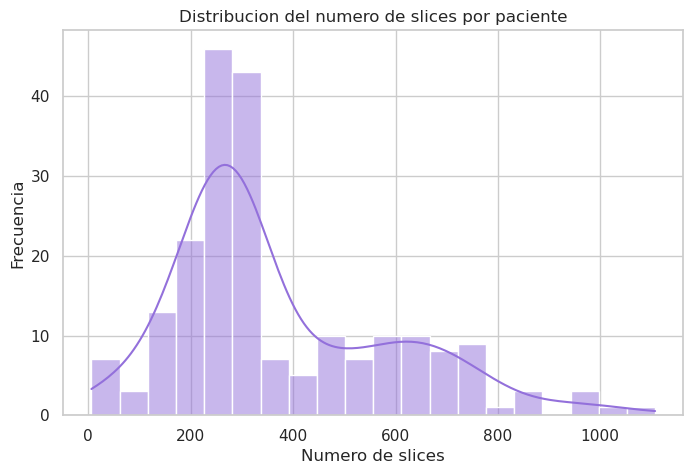
\includegraphics[width=1\textwidth]{imagenes/eda/distribucion_numero_cortes_ct_principal.png}
    \caption{Distribución del número de cortes de los volúmenes de TC.}
    \label{fig:eda_tc_num_cortes}
\end{figure}

% Además del número de cortes, se analizaron otras características espaciales de los volúmenes, como la resolución en plano, el espaciado entre cortes y el volumen de voxel. La Figura~\ref{fig:eda_dicom_heterogeneidad} resume la heterogeneidad espacial observada en las TC principales. La resolución en plano estuvo dominada por matrices de $512 \times 512$ y $768 \times 768$, con 140 y 66 estudios respectivamente. El espaciado X/Y presentó una mediana aproximada de 0,72 mm, aunque con valores comprendidos entre 0,35 y 1,00 mm. Por su parte, el espaciado Z estimado tuvo una mediana de 1,00 mm, con un rango intercuartílico entre 0,68 y 1,25 mm, aunque se observaron casos extremos de hasta 7 mm.

% El volumen de voxel también mostró una variabilidad notable, con una mediana de 0,38 mm$^3$, un rango intercuartílico entre 0,25 y 0,70 mm$^3$ y un valor máximo de 4,43 mm$^3$. Esta variabilidad es especialmente relevante en el contexto de modelos 3D y análisis radiómico, ya que las texturas y patrones espaciales pueden depender del tamaño de voxel y del grosor de corte. Por tanto, estos resultados justifican la aplicación posterior de técnicas de remuestreo espacial y redimensionamiento de los volúmenes.

También se han observado diferencias en la resolución en plano, el espaciado entre cortes y el volumen del vóxel, resumidas en la Figura~\ref{fig:eda_dicom_heterogeneidad}. Las matrices más frecuentes han sido de $512 \times 512$ y $768 \times 768$, mientras que el espaciado X/Y ha presentado una mediana aproximada de 0,72 mm y el espaciado Z una mediana de 1,00 mm. El volumen del vóxel ha alcanzado una mediana de 0,38 mm$^3$, con casos extremos asociados a estudios de menor resolución. Esta heterogeneidad ha justificado el remuestreo y el redimensionado posteriores.

\begin{figure}[!htbp]
    \centering
    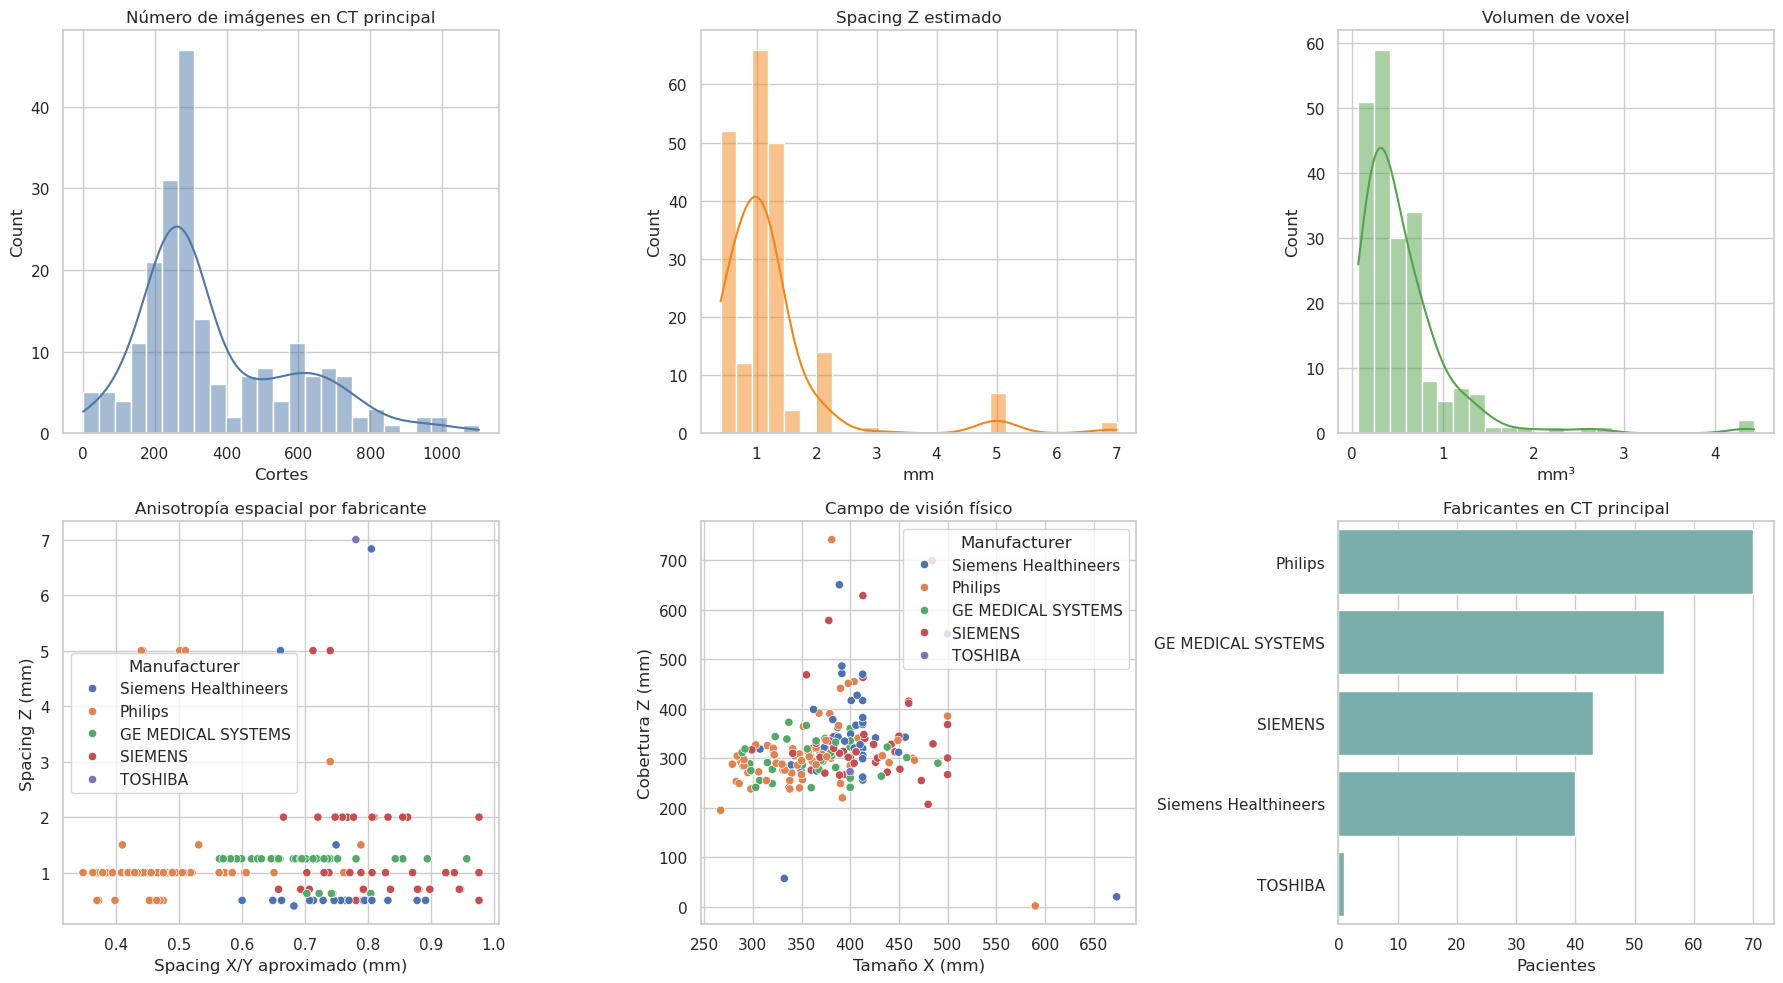
\includegraphics[width=1\textwidth]{imagenes/eda/heterogeneidad_espacial_ct_principal.png}
    \caption{Resumen de la heterogeneidad espacial de las TC principales: número de cortes, espaciado Z, volumen de vóxel, anisotropía espacial, campo de visión físico y distribución por fabricante.}
    \label{fig:eda_dicom_heterogeneidad}
\end{figure}

Los metadatos también han mostrado variabilidad entre fabricantes, modelos de escáner, algoritmos de reconstrucción, valores de kVp, exposición y grosor de corte. Estas diferencias pueden alterar de forma sistemática la resolución, las intensidades y las características de textura de las imágenes, haciendo que los estudios adquiridos con distintos equipos o protocolos presenten variaciones de origen técnico y no biológico. Por ello, constituyen una posible fuente de heterogeneidad y confusión para los modelos.

Las intensidades se han convertido a unidades HU. A continuación, se han calculado estadísticos robustos sobre cortes muestreados de cada estudio. Como muestra la Figura~\ref{fig:eda_dicom_hu}, la mediana de \texttt{HU\_p50} ha sido aproximadamente de $-877$ HU, mientras que las intensidades superiores han reflejado la presencia de tejidos blandos y estructuras de mayor densidad.

\begin{figure}[!htbp]
    \centering
    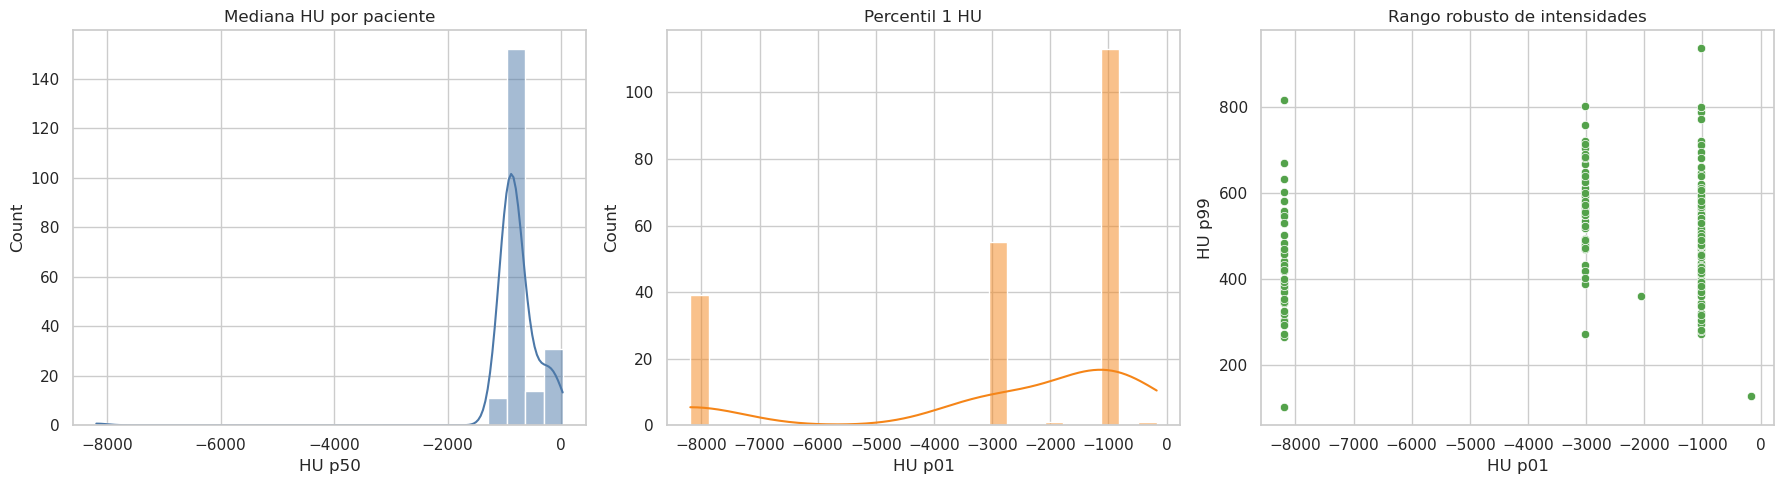
\includegraphics[width=1\textwidth]{imagenes/eda/intensidades_hu.png}
    \caption{Análisis exploratorio de intensidades HU: distribución de la mediana HU por paciente, percentil 1 HU y rango robusto de intensidades entre \texttt{HU\_p01} y \texttt{HU\_p99}.}
    \label{fig:eda_dicom_hu}
\end{figure}

El análisis ha permitido detectar un estudio con intensidades atípicas y dos casos con un número de cortes insuficiente para representar un volumen tridimensional completo. Además, se ha realizado una inspección visual de estudios con características extremas y de una muestra aleatoria, ilustrada en la Figura~\ref{fig:eda_dicom_control_visual}, para comprobar que las series seleccionadas correspondían a TC torácicas coherentes.

\begin{figure}[!htbp]
    \centering
    \includegraphics[width=\textwidth]{imagenes/eda/control_visual_calidad_ct.png}
    \caption{Control visual de calidad mediante cortes centrales de TC principales seleccionadas. Se incluyen ejemplos de pacientes con pocos cortes, muchos cortes, espaciado Z elevado y casos seleccionados aleatoriamente.}
    \label{fig:eda_dicom_control_visual}
\end{figure}

Finalmente, se cruzó la información de las TC principales con los datos clínicos disponibles. La cobertura clínica ha sido completa para los 210 pacientes y se han obtenido 209 pacientes con una TC principal y datos clínicos asociados. Se ha analizado de forma exploratoria si las principales características de adquisición variaban entre los pacientes con hemorragia, con neumotórax o sin ninguna de estas complicaciones. Como se muestra en la Figura~\ref{fig:eda_dicom_cruce_complicacion}, no se ha observado una separación clara entre estos grupos en cuanto al número de cortes ni al espaciado en el eje Z.

\begin{figure}[!htbp]
    \centering
    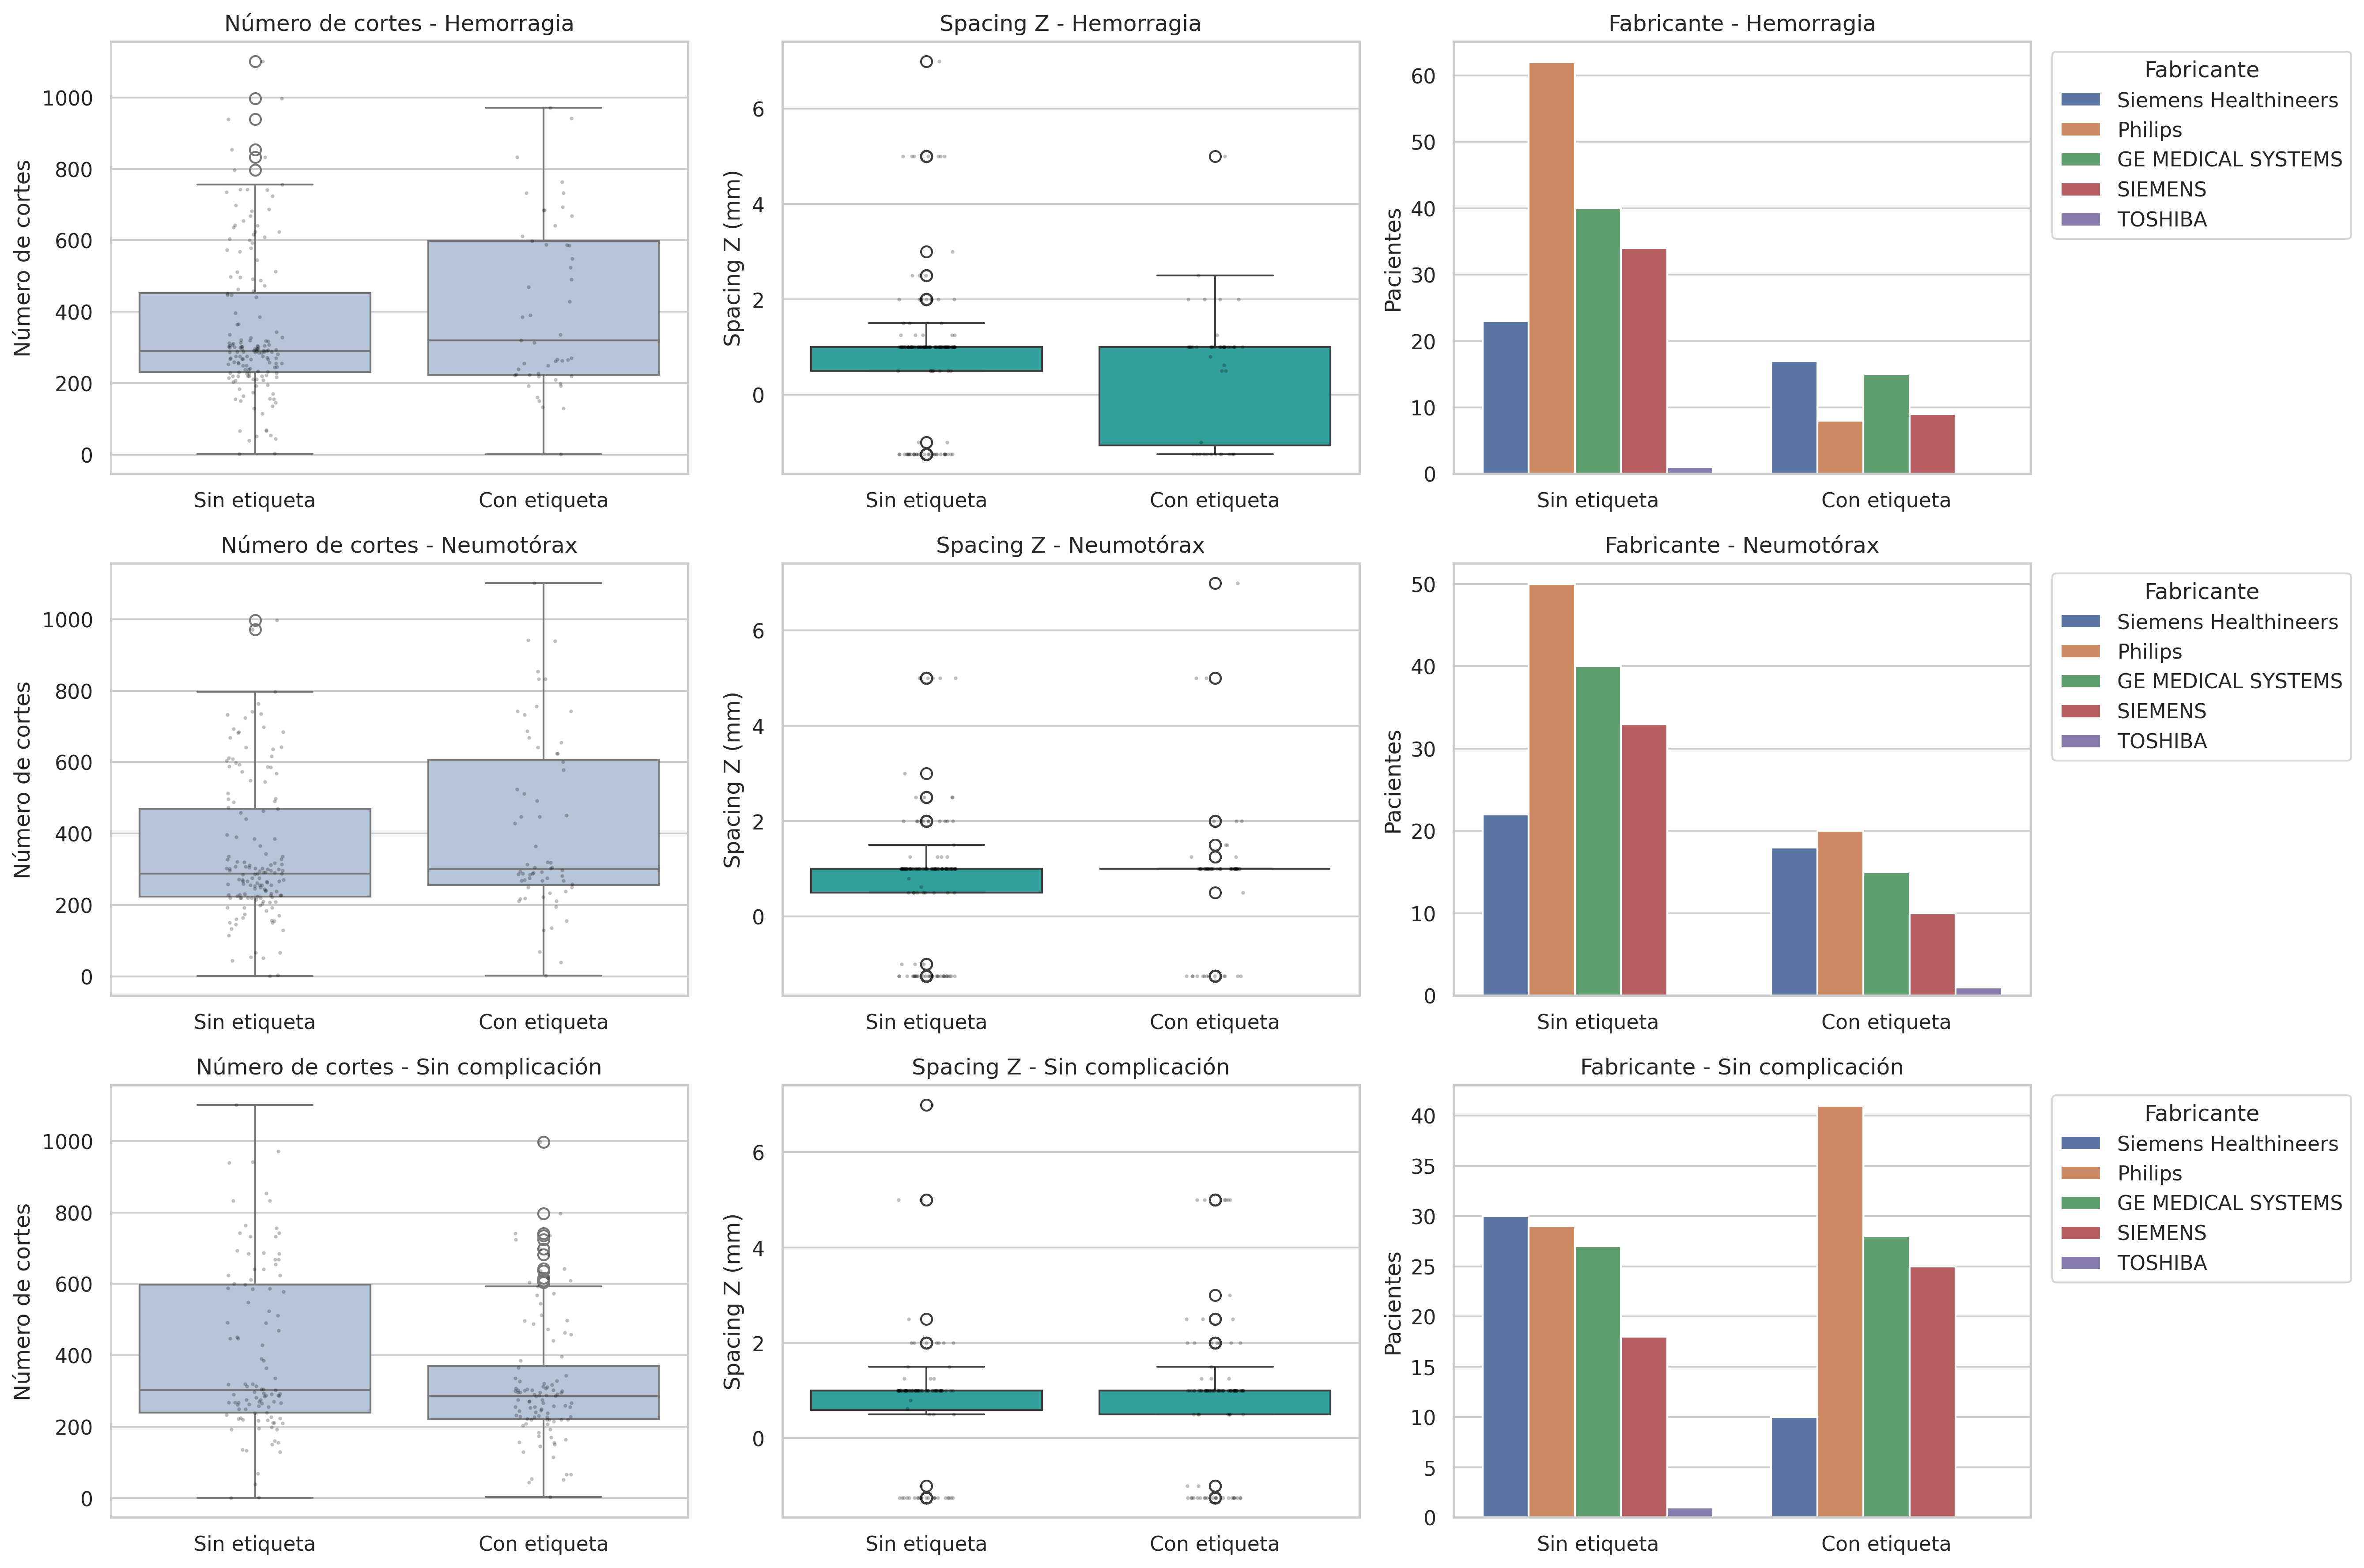
\includegraphics[width=1.2\textwidth]{imagenes/eda/cruce_dicom_etiquetas_complicacion.png}
    \caption{Cruce exploratorio entre características de adquisición DICOM y las principales etiquetas clínicas de complicación. Para cada etiqueta se comparan los pacientes en los que dicha etiqueta está ausente o presente, considerando el número de cortes, el espaciado Z y el fabricante del escáner.}
    \label{fig:eda_dicom_cruce_complicacion}
\end{figure}

En conjunto, el análisis ha identificado heterogeneidad espacial, variabilidad en los parámetros de adquisición y varios casos problemáticos. Estos resultados han motivado la conversión a NIfTI, el control de calidad, la normalización de intensidades y la homogeneización espacial descritos en la sección siguiente.


%-------------------------------------------%


\subsection{Análisis exploratorio de datos clínicos}

% El conjunto de datos clínicos original proporcionado por el equipo médico incluía información demográfica, clínica y anatomopatológica de cada paciente. Las variables originales eran las siguientes:

% \begin{itemize}
%     \item \textbf{Sexo y edad}: recoge el sexo del paciente y su edad en el momento del estudio.

%     \item \textbf{Tipo de cáncer}: indica el subtipo tumoral diagnosticado.

%     \item \textbf{Complicación}: variable binaria que señala si el paciente presentó o no alguna complicación.

%     \item \textbf{Tipo de complicación}: especifica la complicación observada en los casos positivos.

%     \item \textbf{Factor de riesgo}: recoge antecedentes, tratamientos o condiciones clínicas relevantes del paciente.

%     \item \textbf{Patología pulmonar}: describe la presencia de enfermedades respiratorias previas.

%     \item \textbf{Extensión al diagnóstico}: indica si existía extensión de la enfermedad en el momento del diagnóstico.

%     \item \textbf{TC}: identifica la máquina con la que se ha realizado la tomografía computarizada.

%     \item \textbf{Extensión a los 1-5 años}: recoge información de seguimiento posterior del paciente.

%     \item \textbf{Anticoagulación}: indica la presencia de tratamiento anticoagulante o antiagregante.

%     \item \textbf{Mutación}: contiene información molecular o marcadores asociados al tumor.
% \end{itemize}

Como se describió en el Capítulo~\ref{chap:planteamiento_problema}, el conjunto clínico original proporcionado por el equipo médico incluye información demográfica, clínica, anatomopatológica y de complicaciones asociada a cada paciente.

Aunque algunas variables del conjunto original resultan útiles para describir clínicamente la cohorte, no todas son adecuadas como entradas predictivas. En particular, se excluyeron de las fases de modelado aquellas variables conocidas únicamente después de la biopsia o durante el seguimiento posterior, ya que su uso introduciría información no disponible en el momento de la predicción. Entre ellas se encuentran \textit{Extensión al diagnóstico}, \textit{TC}, \textit{Extensión a los 1-5 años}, \textit{Anticoagulación} y \textit{Mutación}. Además, la variable \textit{Tipo de cáncer} se conservó únicamente durante el análisis exploratorio, al aportar contexto clínico sobre la cohorte, pero no se utilizó posteriormente como variable predictora.

Tras la selección inicial, se ha conservado para el análisis exploratorio el siguiente subconjunto de las variables descritas en la Sección~\ref{sec:variables_disponibles}:

% \begin{itemize}
%     \item \textbf{Identificador del paciente}: código único asignado a cada paciente, utilizado únicamente para mantener la trazabilidad de los casos.

%     \item \textbf{Sexo}: variable categórica que indica el sexo del paciente.

%     \item \textbf{Edad}: variable numérica que recoge la edad del paciente.

%     \item \textbf{Tipo de cáncer}: variable categórica que describe el subtipo tumoral diagnosticado. Se conserva en esta fase para caracterizar la cohorte durante el análisis exploratorio.

%     \item \textbf{Complicación}: variable objetivo en clasificación binaria que indica si el paciente presentó o no alguna complicación. En este trabajo no es utilizada para modelar.

%     \item \textbf{Tipo de complicación}: variable que especifica el tipo de complicación observada en los pacientes con complicación. Es una variable de texto multietiqueta, ya que puede contener varias complicaciones para un mismo paciente.

%     \item \textbf{Factor de riesgo}: variable de texto multietiqueta que recoge antecedentes, tratamientos o condiciones clínicas relevantes.

%     \item \textbf{Patología pulmonar}: variable de texto multietiqueta con condiciones respiratorias previas.
% \end{itemize}
\begin{itemize}
    \item \textbf{Identificación}: identificador del paciente.
    \item \textbf{Variables demográficas}: sexo y edad.
    \item \textbf{Diagnóstico oncológico}: tipo de cáncer.
    \item \textbf{Complicaciones}: presencia y tipo de complicación.
    \item \textbf{Antecedentes clínicos}: factores de riesgo y patologías pulmonares.
\end{itemize}

Estas variables constituyen el conjunto utilizado para el análisis exploratorio inicial. Posteriormente, durante la fase de preprocesamiento, algunas de ellas fueron transformadas o eliminadas para obtener una representación adecuada para el entrenamiento de los modelos. Tras dicho procesamiento, el conjunto de datos quedó formado por 210 pacientes y 52 columnas, sin valores nulos y con un identificador único para cada paciente.

En primer lugar, se analizó el perfil oncológico de la cohorte a partir de la variable \textit{Tipo de cáncer}. Aunque esta variable no se utiliza posteriormente como entrada del modelo, resulta útil para contextualizar clínicamente el conjunto de pacientes. Como se observa en la Figura~\ref{fig:eda_tipos_cancer}, el subtipo dominante es el adenocarcinoma, seguido del carcinoma epidermoide y de un grupo de pacientes en los que el tipo tumoral no aparece especificado.

\begin{figure}[htbp]
    \centering
    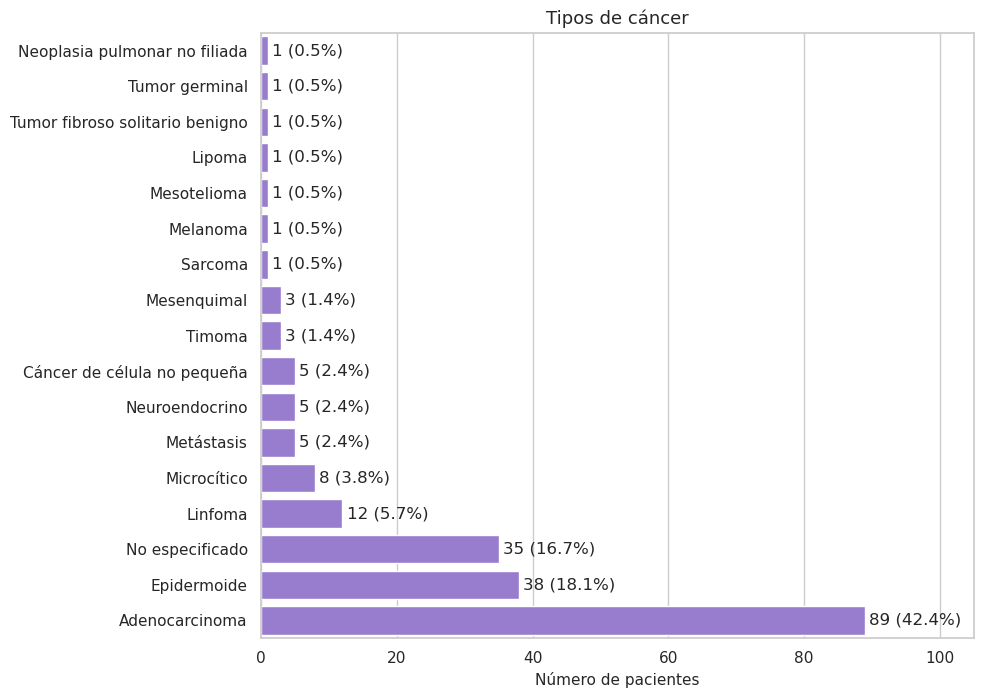
\includegraphics[width=1\textwidth]{imagenes/eda/tipos_cancer.png}
    \caption{Distribución de los tipos de cáncer presentes en la cohorte clínica.}
    \label{fig:eda_tipos_cancer}
\end{figure}

% También se estudió la proporción de complicación en función del tipo de cáncer, tal y como se muestra en la Figura~\ref{fig:eda_tasa_complicacion_tipo_cancer}. Para evitar interpretaciones poco fiables, el gráfico se restringió a aquellas categorías con al menos cinco pacientes. El adenocarcinoma es el grupo mayoritario, con 89 pacientes y una tasa de complicación del 61,8~\%. Le siguen el tipo epidermoide, con 38 pacientes y una tasa del 42,1~\%, y el grupo no especificado, con 35 pacientes y una tasa del 48,6~\%. No obstante, estas diferencias deben interpretarse de forma descriptiva, especialmente en las categorías con menor soporte.

% \begin{figure}[htbp]
%     \centering
%     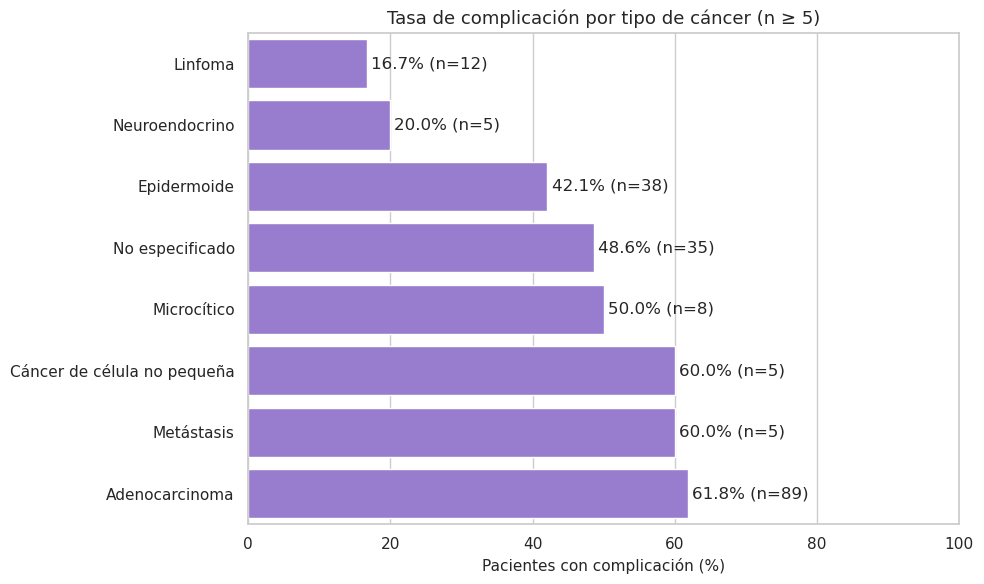
\includegraphics[width=1\textwidth]{imagenes/eda/tasa_complicacion_tipo_cancer.png}
%     \caption{Tasa de complicación por tipo de cáncer para las categorías con al menos cinco pacientes.}
%     \label{fig:eda_tasa_complicacion_tipo_cancer}
% \end{figure}

A continuación, se analizó el soporte de las complicaciones registradas en la cohorte clínica inicial. Como se muestra en la Figura~\ref{fig:eda_soporte_etiquetas}, el neumotórax fue la complicación más frecuente, con 64 casos, seguido de la hemorragia, con 49. El derrame pleural se registró únicamente en un paciente, por lo que no se incorporó como objetivo debido a su soporte insuficiente. Este caso se mantuvo en la caracterización descriptiva de la cohorte, pero se excluyó de los análisis centrados en las complicaciones modeladas.

Tras esta exclusión, la cohorte elegible para la formulación multietiqueta estuvo compuesta por 209 pacientes. Hemorragia y neumotórax se consideraron como las dos salidas del estudio y coexistieron en 9 pacientes. El estado derivado \textit{Sin complicación} incluyó 105 pacientes en los que no se registró ninguno de estos dos eventos.

\begin{figure}[!htbp]
    \centering
    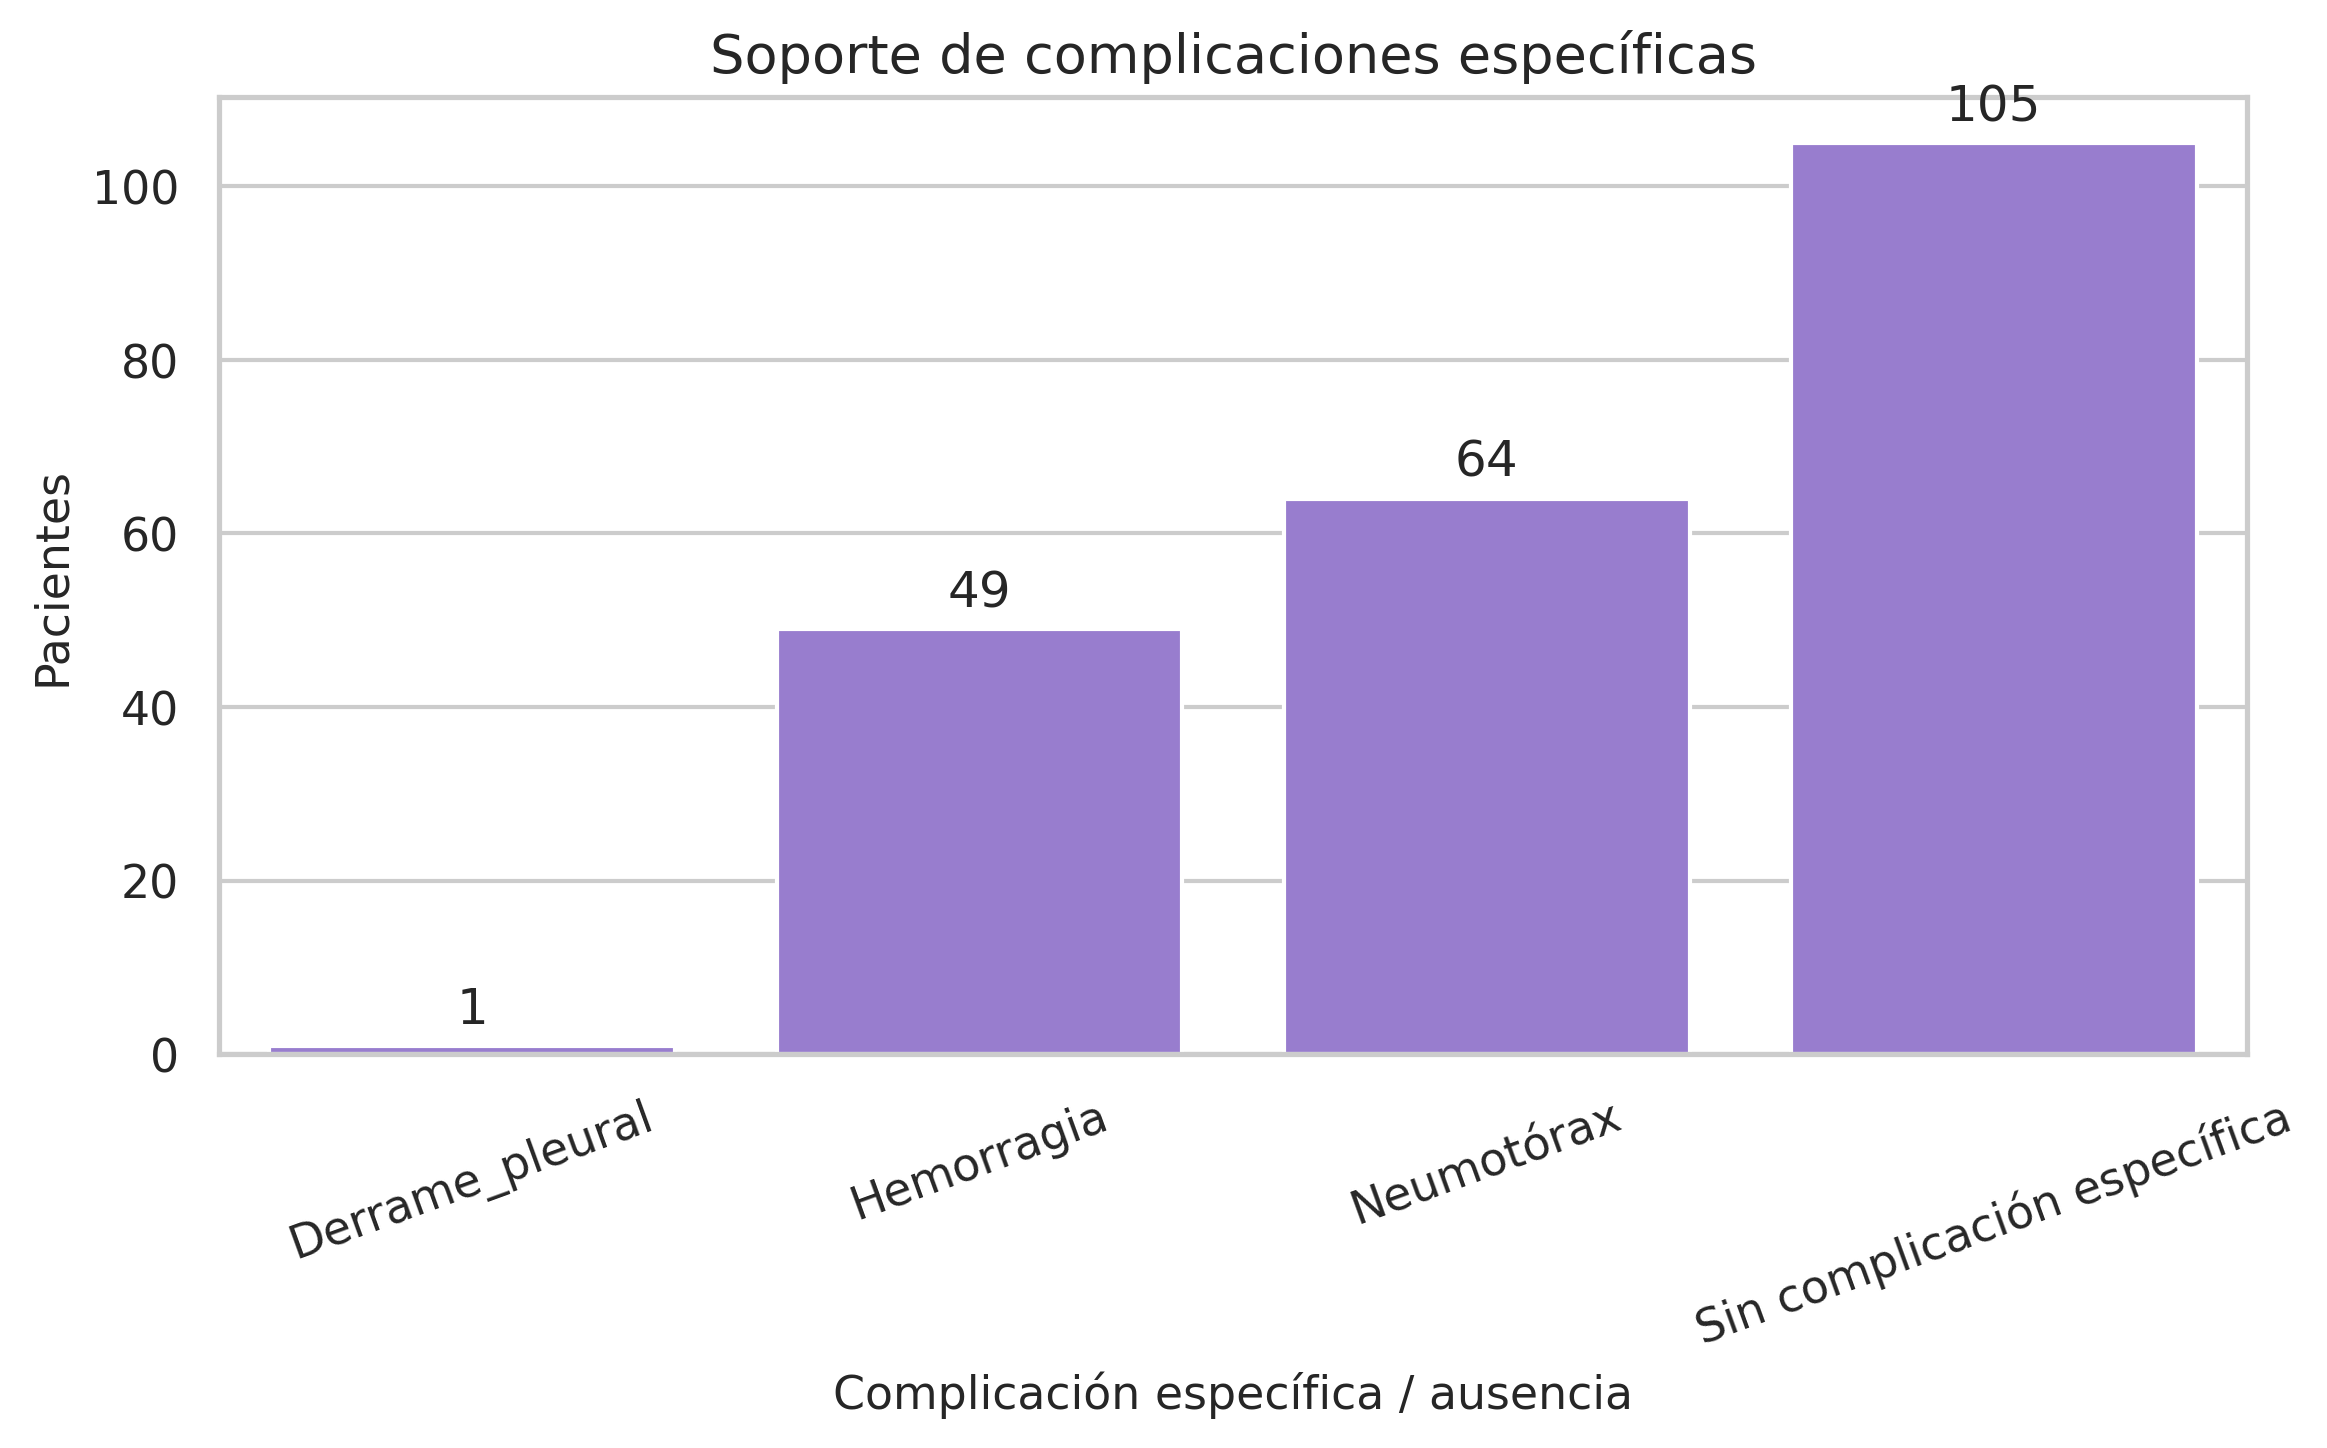
\includegraphics[width=1\textwidth]{imagenes/eda/soporte_etiquetas_complicaciones.png}
    \caption{Soporte de las complicaciones registradas y de la ausencia de complicaciones en la cohorte clínica inicial.}
    \label{fig:eda_soporte_etiquetas}
\end{figure}

La Figura~\ref{fig:eda_numero_complicaciones} resume el número de tipos de complicación registrados por paciente.

\begin{figure}[!htbp]
    \centering
    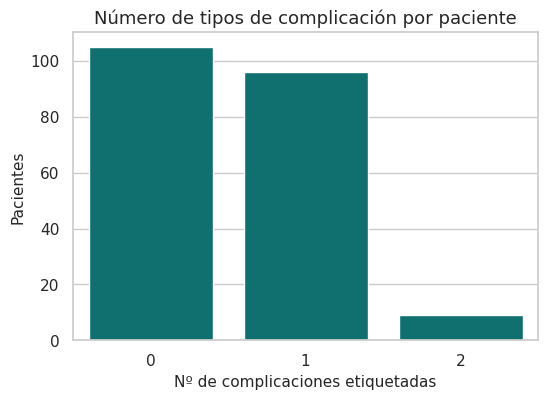
\includegraphics[width=0.7\textwidth]{imagenes/eda/numero_complicaciones_por_paciente.png}
    \caption{Número de tipos de complicación etiquetados por paciente.}
    \label{fig:eda_numero_complicaciones}
\end{figure}

Para completar el análisis multietiqueta, se estudió la coocurrencia entre complicaciones específicas. La matriz de la Figura~\ref{fig:eda_coocurrencia_complicaciones} muestra que la única coocurrencia relevante se produce entre \textit{Hemorragia} y \textit{Neumotórax}, con 9 pacientes que presentan ambas complicaciones. El \textit{Derrame pleural}, al estar presente en un único paciente, no muestra coocurrencia con el resto de etiquetas.

\begin{figure}[!htbp]
    \centering
    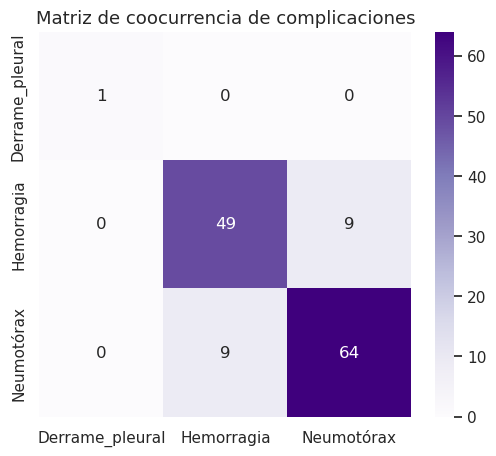
\includegraphics[width=0.7\textwidth]{imagenes/eda/coocurrencia_complicaciones.png}
    \caption{Matriz de coocurrencia entre las complicaciones específicas.}
    \label{fig:eda_coocurrencia_complicaciones}
\end{figure}

Desde el punto de vista demográfico, se analizó en primer lugar la edad, al ser la única variable cuantitativa de la cohorte. En la Figura~\ref{fig:eda_edad_distribucion_complicacion} se muestra su distribución global en años y su comparación descriptiva entre los pacientes positivos para las principales etiquetas de complicación. La mayor parte de las observaciones se concentra aproximadamente entre los 60 y los 80 años, con una cola hacia edades más jóvenes, lo que refleja una cohorte formada mayoritariamente por pacientes de edad avanzada. Los diagramas de caja muestran un solapamiento considerable entre \textit{Hemorragia}, \textit{Neumotórax} y \textit{Sin complicación}. Las dos complicaciones presentan medianas ligeramente superiores a la ausencia de complicación, aunque no se aprecia una separación clara entre los subconjuntos.

\begin{figure}[!htbp]
    \centering
    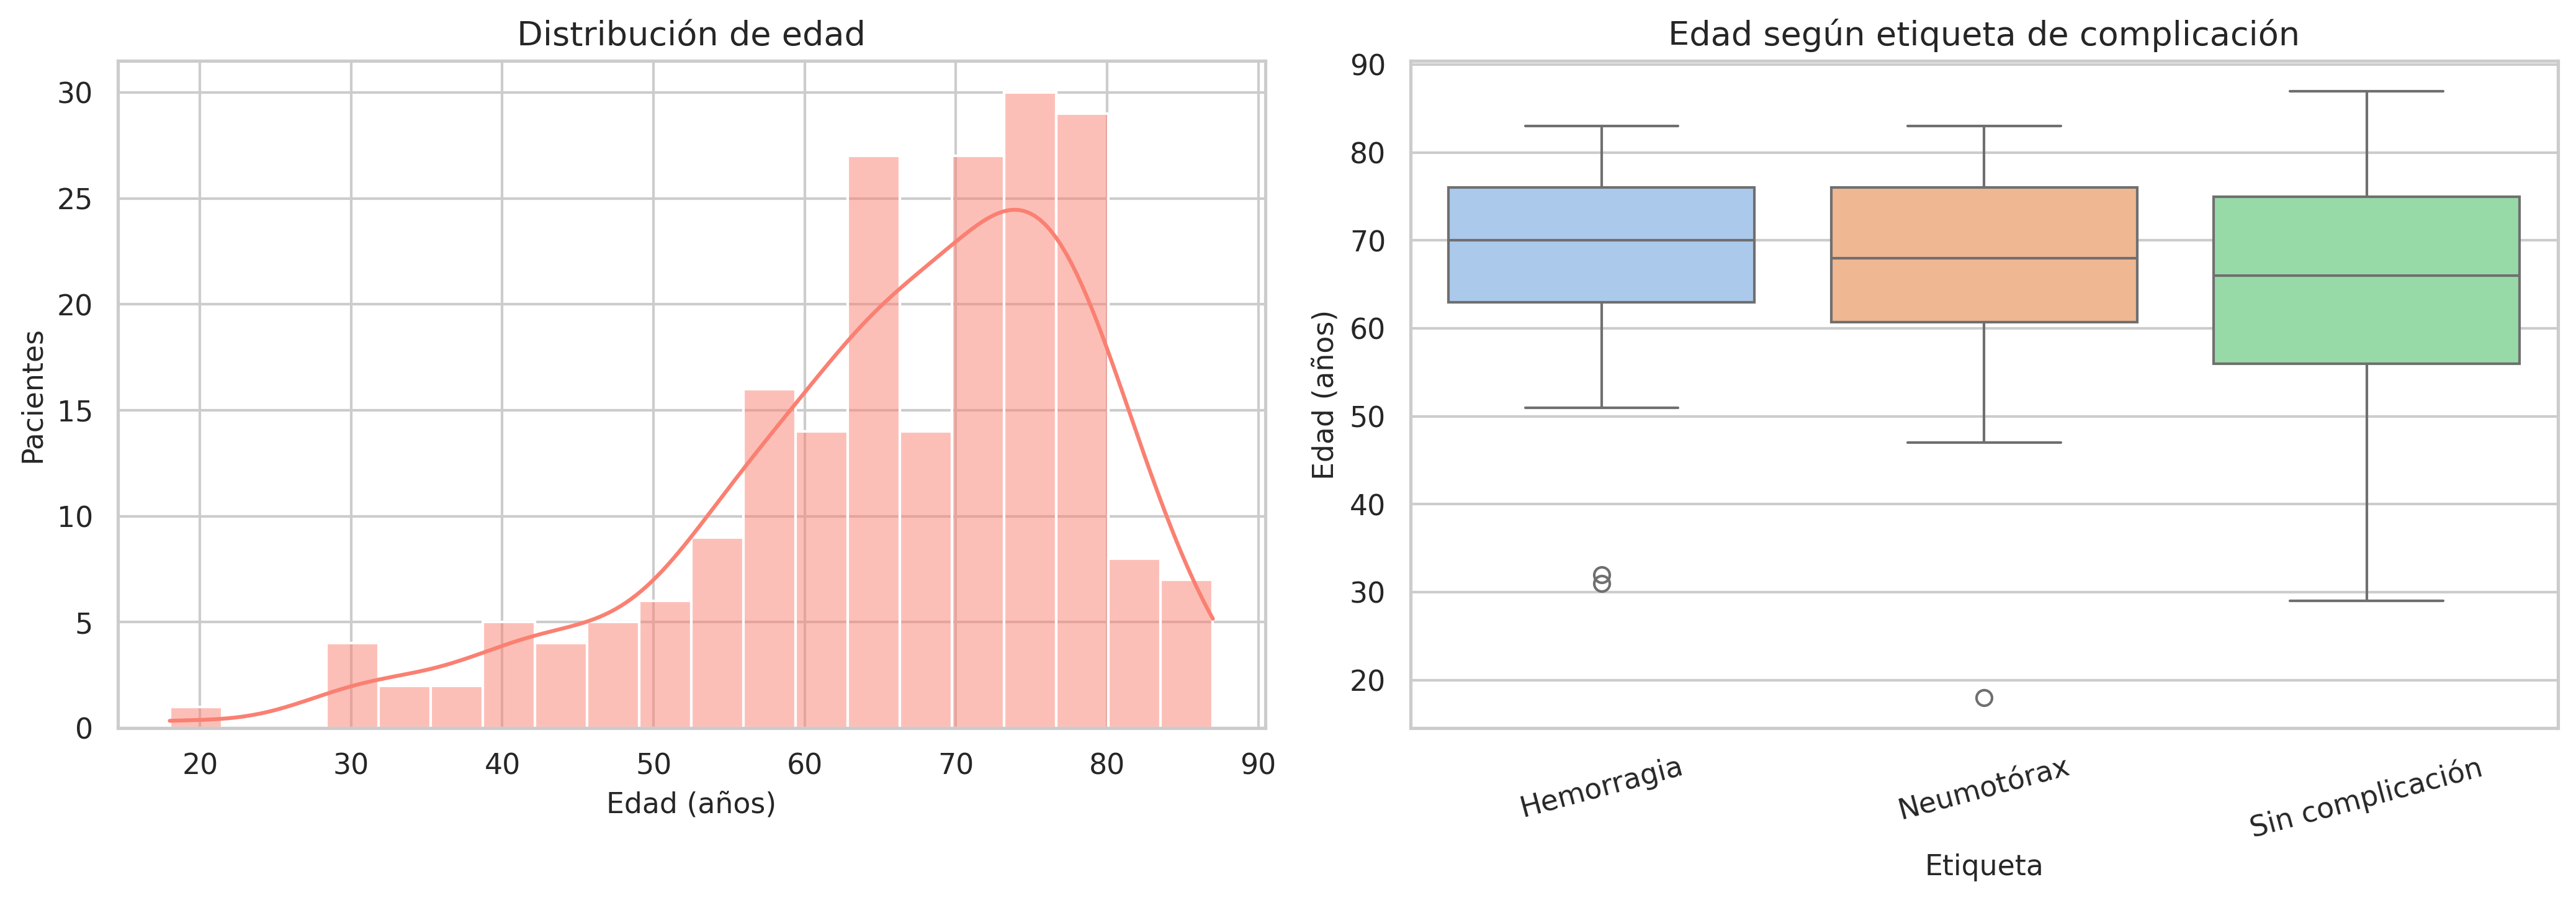
\includegraphics[width=1\textwidth]{imagenes/eda/edad_sin_normalizar_hist_boxplot_complicacion.png}
    \caption{Distribución global de la edad en la cohorte y comparación descriptiva según las principales etiquetas de complicación. El panel izquierdo muestra la distribución de la edad en años y el panel derecho presenta los diagramas de caja correspondientes a hemorragia, neumotórax y ausencia de ambas complicaciones.}
    \label{fig:eda_edad_distribucion_complicacion}
\end{figure}

Además, se realizó un análisis univariante más detallado de la edad mediante estadísticos robustos y la distribución acumulada, representados en la Figura~\ref{fig:eda_resumen_edad}. La mediana de edad fue de 68 años, con un rango intercuartílico entre 59 y 76 años, y un rango total comprendido entre 18 y 87 años. La media fue de 66,0 años, ligeramente inferior a la mediana, lo que concuerda con una ligera asimetría hacia edades más jóvenes. El test de Shapiro-Wilk rechazó la normalidad exacta, por lo que la edad se describió combinando media y desviación estándar con mediana y rango intercuartílico. Los valores extremos detectados correspondían a pacientes jóvenes, pero se consideraron observaciones clínicamente plausibles y no fueron eliminados, especialmente teniendo en cuenta el tamaño reducido de la cohorte.

\begin{figure}[!htbp]
    \centering
    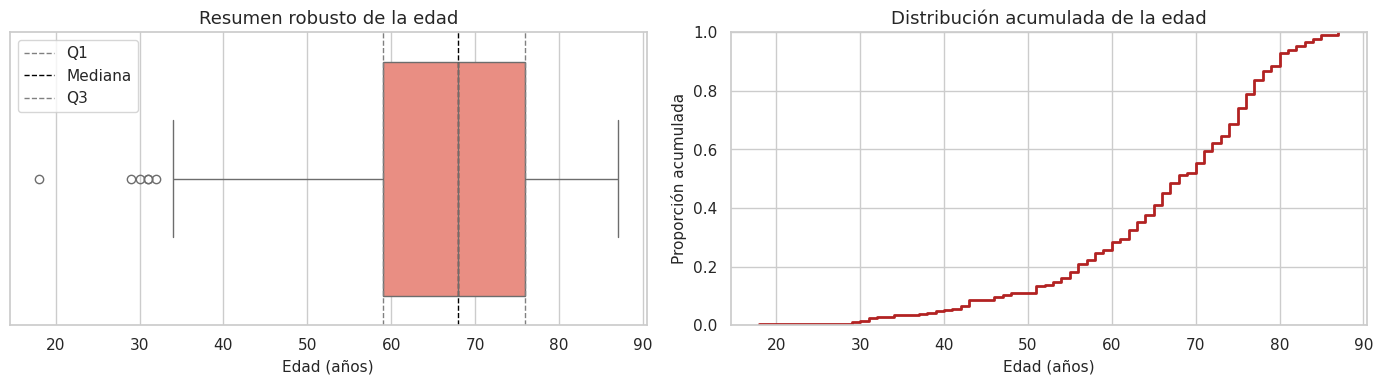
\includegraphics[width=1\textwidth]{imagenes/eda/resumen_robusto_edad_ecdf.png}
    \caption{Resumen robusto de la edad y distribución acumulada de la edad.}
    \label{fig:eda_resumen_edad}
\end{figure}

También se agrupó la edad en intervalos únicamente con finalidad descriptiva. Como se muestra en la Figura~\ref{fig:eda_grupos_edad}, los grupos más representados son los de 60 a 69 años y 70 a 79 años, lo que confirma la concentración de la cohorte en edades avanzadas. 

\begin{figure}[!htbp]
    \centering
    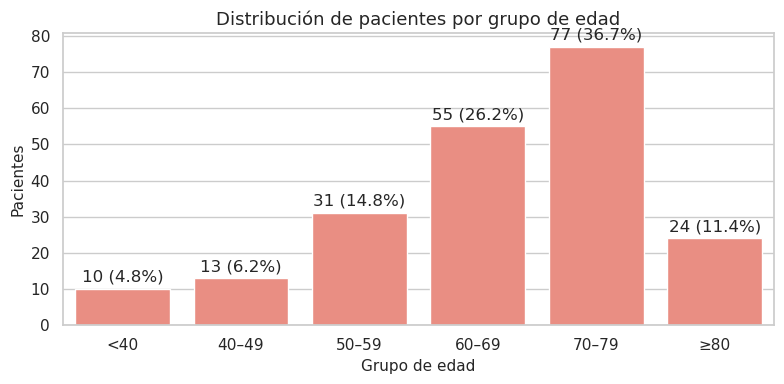
\includegraphics[width=0.9\textwidth]{imagenes/eda/grupos_edad.png}
    \caption{Distribución de pacientes por grupo de edad.}
    \label{fig:eda_grupos_edad}
\end{figure}


Como complemento, la Figura~\ref{fig:eda_complicaciones_grupos_edad} muestra la proporción de pacientes con cada resultado dentro de los distintos grupos de edad. En los grupos menores de 50 años predomina el estado sin complicación, mientras que a partir de los 50 años aumenta la proporción de complicaciones, especialmente de neumotórax. La hemorragia presenta una distribución más estable entre los grupos de mayor edad. Estas diferencias deben interpretarse de forma descriptiva, ya que los grupos de menor edad contienen pocos pacientes. 

\begin{figure}[!htbp]
    \centering
    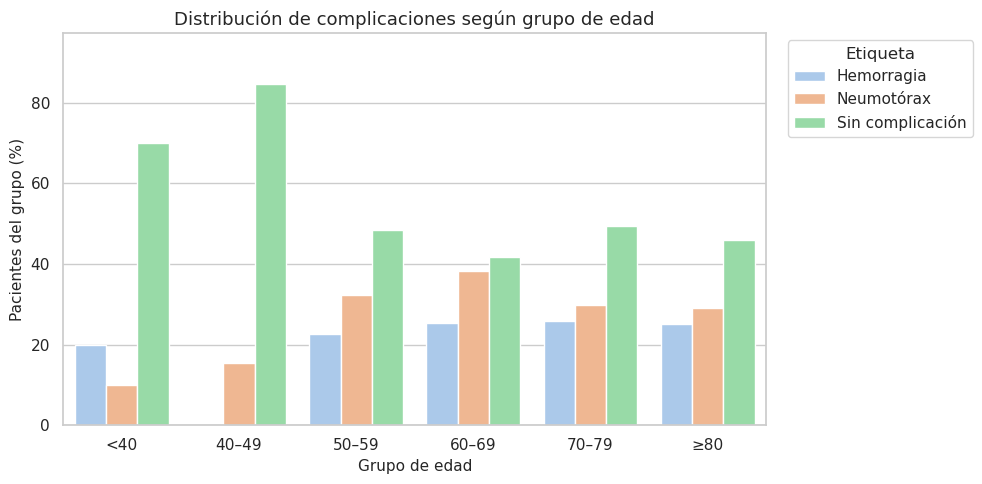
\includegraphics[width=\textwidth]{imagenes/eda/distribucion_edades_etiquetas.png}
    \caption{Proporción de pacientes con hemorragia, neumotórax y ausencia de ambas complicaciones dentro de cada grupo de edad.}
    \label{fig:eda_complicaciones_grupos_edad}
\end{figure}



Respecto al sexo, se observa una mayor presencia de hombres que de mujeres, con 135 hombres frente a 75 mujeres, lo que equivale al 64,3~\% y 35,7~\% del total, respectivamente. Esta distribución se representa en la Figura~\ref{fig:eda_sexo_complicacion}. Al analizar las etiquetas de forma independiente, la hemorragia fue ligeramente más frecuente en mujeres, con un 25,3~\% frente al 22,2~\% en hombres, mientras que el neumotórax presentó una mayor proporción en hombres, con un 33,3~\% frente al 25,3~\% en mujeres. La etiqueta sin complicación fue más frecuente en mujeres, con un 54,7~\% frente al 47,4~\% en hombres. Desde el punto de vista clínico, el equipo médico señaló que la mayor proporción de hombres podría estar relacionada con una mayor exposición histórica al tabaco en la población masculina, especialmente en generaciones anteriores.


\begin{figure}[!htbp]
    \centering
    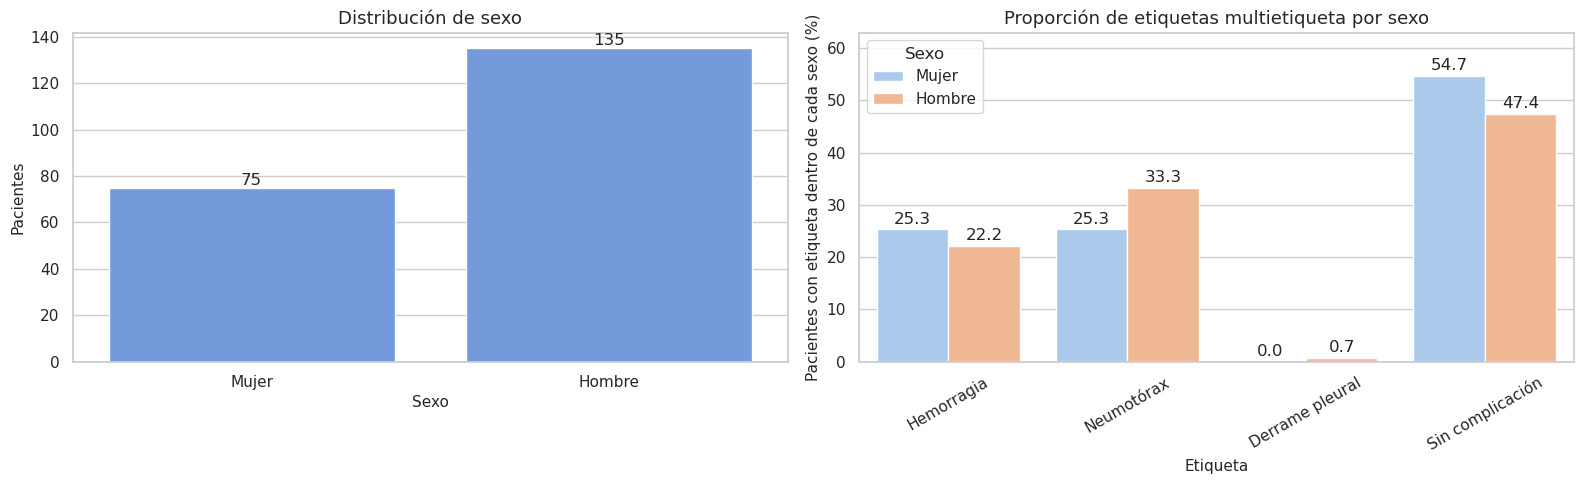
\includegraphics[width=1\textwidth]{imagenes/eda/sexo_complicaciones.png}
    \caption{Distribución de pacientes por sexo y proporción de etiquetas multietiqueta dentro de cada grupo.}
    \label{fig:eda_sexo_complicacion}
\end{figure}

% Posteriormente, se estudió la prevalencia de las variables clínicas y patológicas binarias generadas tras la codificación de las variables multietiqueta. Como se observa en la Figura~\ref{fig:eda_top20_variables}, entre las variables más frecuentes destacan el tabaquismo, presente en 91 pacientes, la hipertensión arterial, presente en 65 pacientes, y el extabaquismo, presente en 63 pacientes. Dentro de las patologías pulmonares, las variables más habituales fueron el enfisema centrolobulillar, el enfisema paraseptal y la hipertensión pulmonar. También se identificaron variables con muy bajo soporte, algunas presentes únicamente en uno, dos o tres pacientes, por lo que su utilidad predictiva debe valorarse con cautela.

% \begin{figure}[!htbp]
%     \centering
%     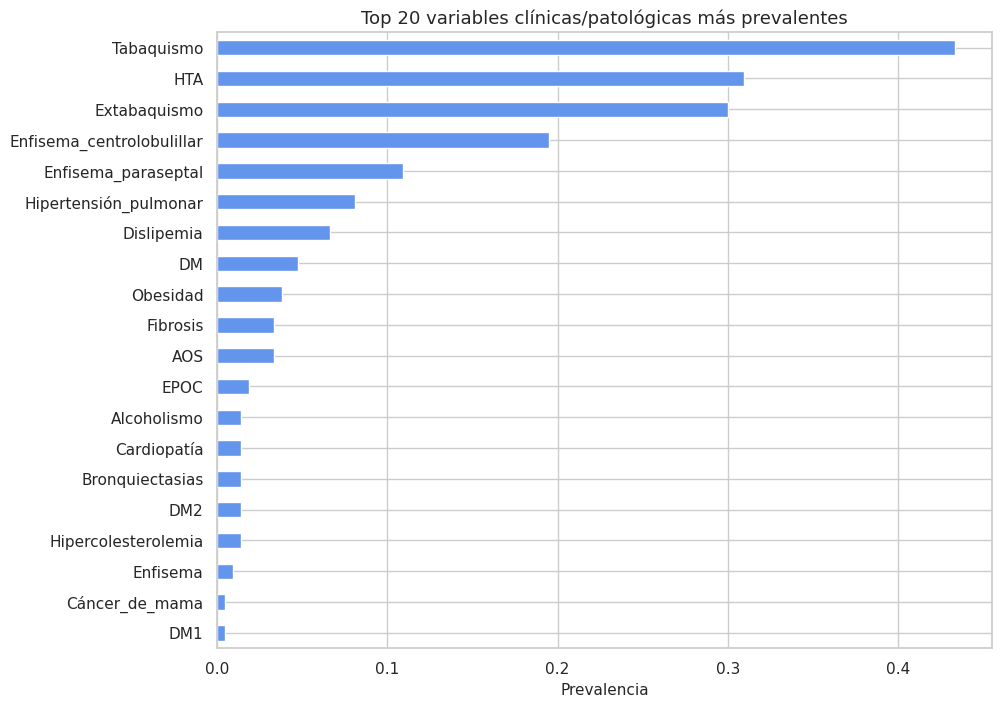
\includegraphics[width=1\textwidth]{imagenes/eda/top20_variables_clinicas_patologicas.png}
%     \caption{Top 20 de variables clínicas y patológicas binarias más prevalentes.}
%     \label{fig:eda_top20_variables}
% \end{figure}

% Para interpretar mejor el origen de estas variables binarias, también se analizaron las categorías originales de patología pulmonar y factor de riesgo. En la Figura~\ref{fig:eda_patologias_originales} se muestran las patologías pulmonares más frecuentes antes de su codificación, excluyendo valores vacíos o marcadores de ausencia. Esta representación permite diferenciar las condiciones respiratorias previas de otros factores clínicos generales.

Posteriormente, se analizaron por separado las categorías originales correspondientes a las variables \textit{Factor de riesgo} y \textit{Patología pulmonar}. Este análisis permite interpretar con mayor claridad qué antecedentes clínicos y qué condiciones respiratorias previas son más frecuentes en la cohorte.

En primer lugar, se analizaron las patologías pulmonares previas. En la Figura~\ref{fig:eda_patologias_originales} se muestran las condiciones respiratorias más frecuentes, excluyendo valores vacíos o marcadores de ausencia. Dentro de este grupo destacan el enfisema centrolobulillar, el enfisema paraseptal y la hipertensión pulmonar.

\begin{figure}[!htbp]
    \centering
    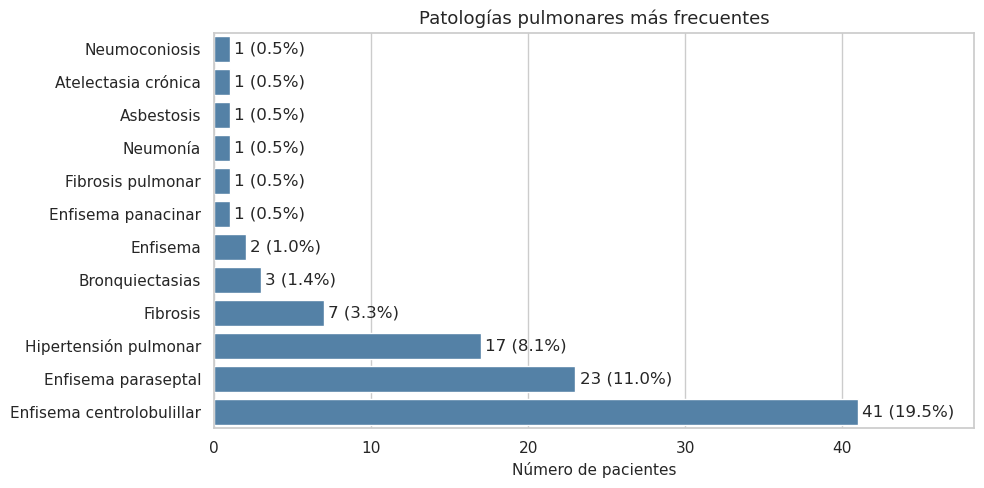
\includegraphics[width=0.9\textwidth]{imagenes/eda/patologias_pulmonares_originales.png}
    \caption{Patologías pulmonares previas más frecuentes en la cohorte clínica.}
    \label{fig:eda_patologias_originales}
\end{figure}

A continuación, se estudiaron los factores de riesgo registrados en el conjunto de datos. Como se observa en la Figura~\ref{fig:eda_factores_riesgo_originales}, entre los más frecuentes destacan el tabaquismo, presente en 91 pacientes, la hipertensión arterial, presente en 65 pacientes, y el extabaquismo, presente en 63 pacientes. Estos factores resultan clínicamente relevantes, ya que reflejan antecedentes habituales en pacientes con cáncer pulmonar y pueden estar relacionados con una mayor vulnerabilidad respiratoria.

\begin{figure}[!htbp]
    \centering
    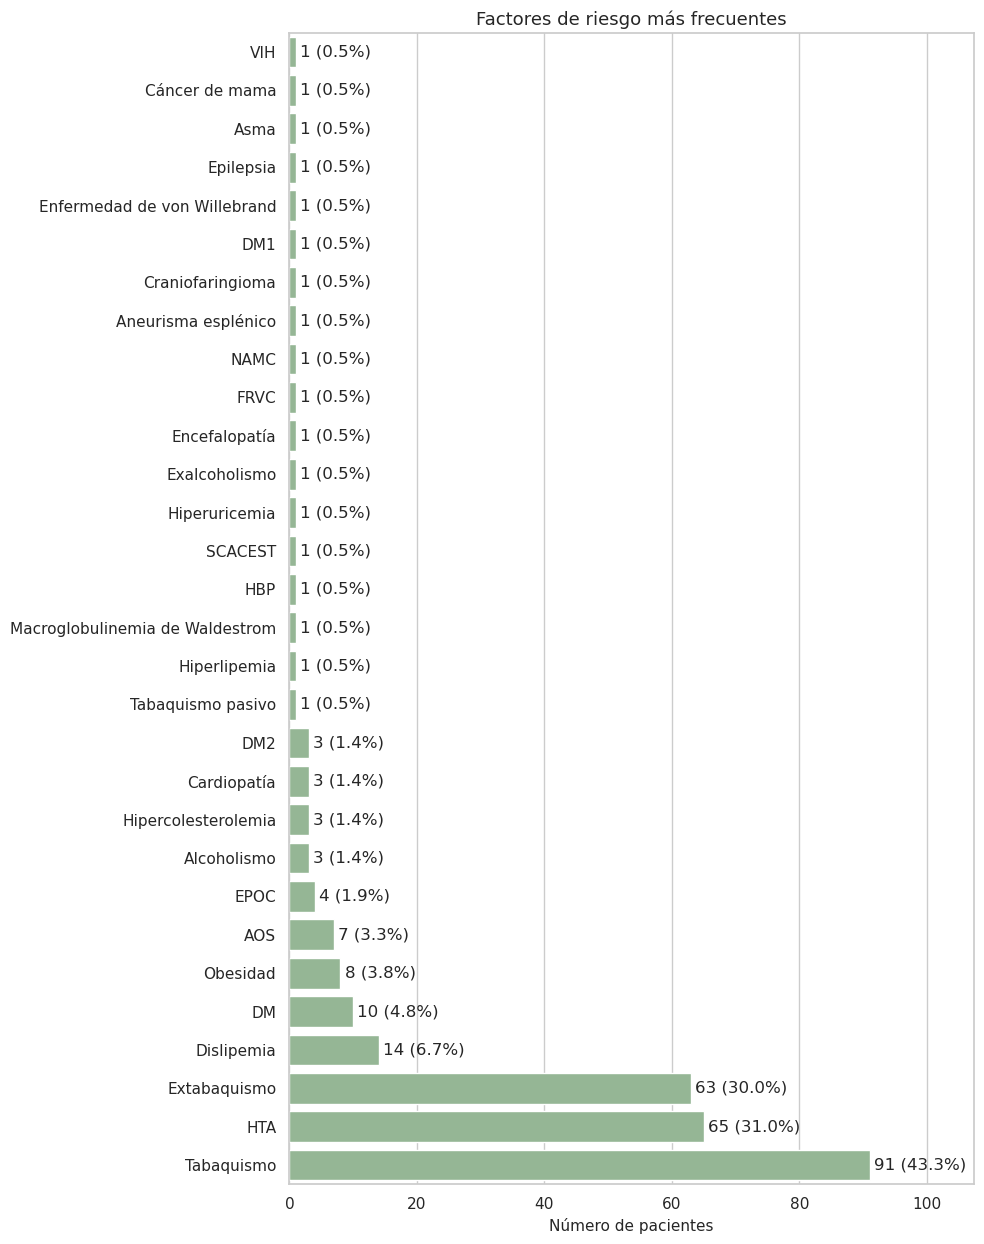
\includegraphics[width=1\textwidth]{imagenes/eda/factores_riesgo_originales.png}
    \caption{Factores de riesgo más frecuentes en las variables clínicas originales.}
    \label{fig:eda_factores_riesgo_originales}
\end{figure}

Finalmente, se exploró la relación entre las variables clínicas y patológicas más prevalentes y la presencia de complicaciones. Para cada variable, se calculó la proporción de pacientes que presentaba cada complicación o ninguna de ellas. Como se muestra en la Figura~\ref{fig:eda_tasa_complicacion_variables}, algunas variables han presentado proporciones elevadas para determinados resultados clínicos. Sin embargo, los porcentajes extremos deben interpretarse teniendo en cuenta el número de pacientes de cada grupo: la EPOC y la hipercolesterolemia solo estaban presentes en cuatro y tres pacientes, respectivamente, por lo que estas proporciones no permiten establecer asociaciones estables.

\begin{figure}[!htbp]
    \centering
    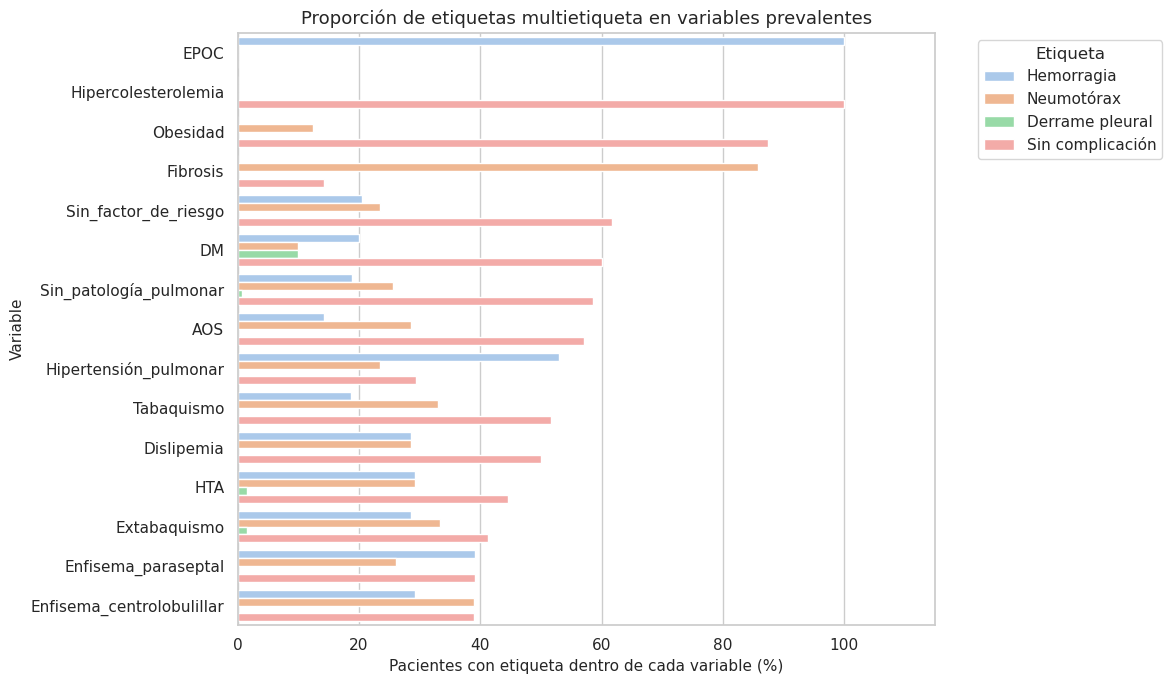
\includegraphics[width=1\textwidth]{imagenes/eda/tasa_complicaciones_variables_prevalentes.png}
    \caption{Proporción de complicaciones y de ausencia de complicación en los pacientes con las variables clínicas y patológicas analizadas.}
    \label{fig:eda_tasa_complicacion_variables}
\end{figure}

Además, se comparó la prevalencia de cada variable entre pacientes con y sin hemorragia, con y sin neumotórax, y según el estado derivado de ausencia de ambas complicaciones. La Figura~\ref{fig:eda_diferencia_prevalencia} muestra las variables con mayor diferencia positiva de prevalencia para cada resultado analizado. En hemorragia destacan la hipertensión pulmonar, la hipertensión arterial, el enfisema paraseptal, el extabaquismo y la EPOC, mientras que en neumotórax aparecen principalmente fibrosis, enfisema centrolobulillar, tabaquismo, bronquiectasias y extabaquismo. En los pacientes sin ninguna de las dos complicaciones, las mayores diferencias se observan para la ausencia de patología pulmonar y de factores de riesgo. El test exacto de Fisher, con corrección por comparaciones múltiples, no identificó asociaciones estadísticamente significativas.

\begin{figure}[!htbp]
    \centering
    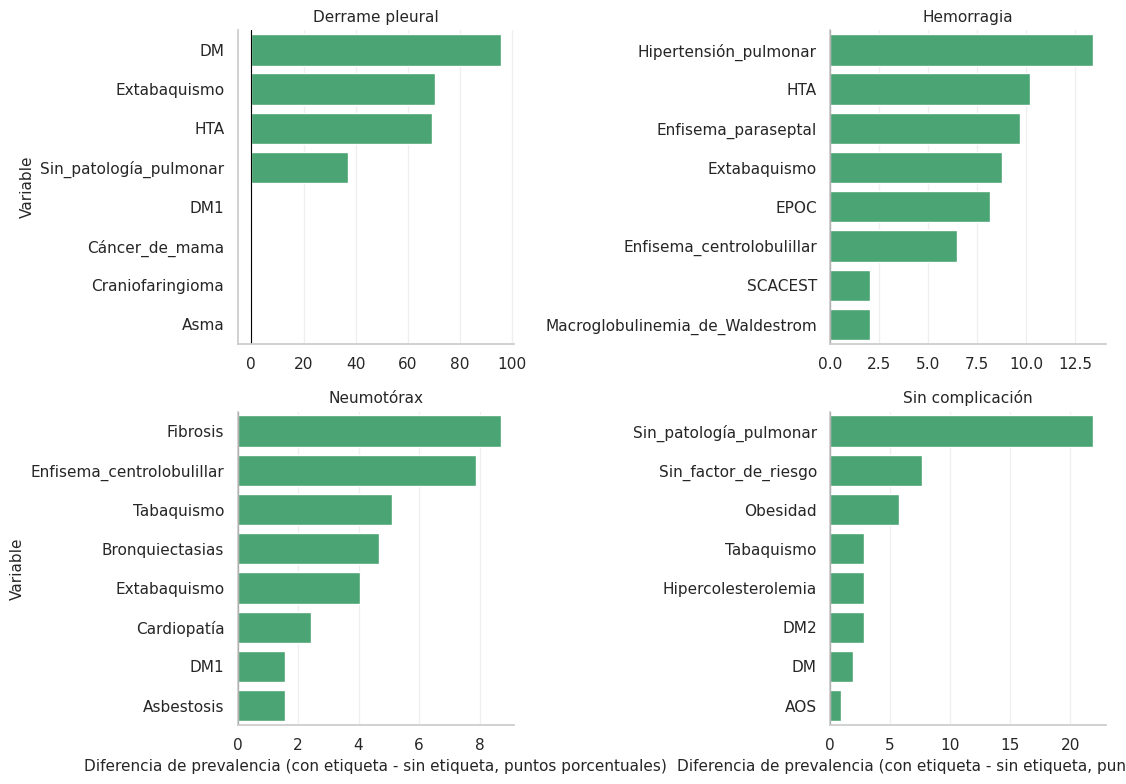
\includegraphics[width=1\textwidth]{imagenes/eda/diferencia_prevalencia_complicaciones.png}
    \caption{Variables con mayor diferencia positiva de prevalencia para hemorragia, neumotórax y el estado derivado de ausencia de ambas complicaciones.}
    \label{fig:eda_diferencia_prevalencia}
\end{figure}

También se compararon de forma exploratoria los perfiles clínicos asociados a las complicaciones específicas más frecuentes, \textit{Hemorragia} y \textit{Neumotórax}. Este análisis sugiere que ambas etiquetas no presentan exactamente el mismo perfil clínico. En los pacientes con hemorragia aparecen con mayor prevalencia variables cardiovasculares y respiratorias como hipertensión pulmonar, hipertensión arterial, enfisema paraseptal, extabaquismo, EPOC y enfisema centrolobulillar. En cambio, en los pacientes con neumotórax destacan fibrosis, enfisema centrolobulillar, tabaquismo, bronquiectasias y extabaquismo. Estas diferencias apoyan la idea de que las complicaciones específicas podrían responder a mecanismos clínicos parcialmente distintos.

Por último, se calculó un mapa de correlaciones exploratorio entre las etiquetas multietiqueta y las variables clínicas más frecuentes. Como se observa en la Figura~\ref{fig:eda_mapa_correlaciones}, no aparecen correlaciones fuertes entre las variables clínicas y las etiquetas, aunque sí se observan algunas relaciones débiles con complicaciones específicas.

\begin{figure}[!htbp]
    \centering
    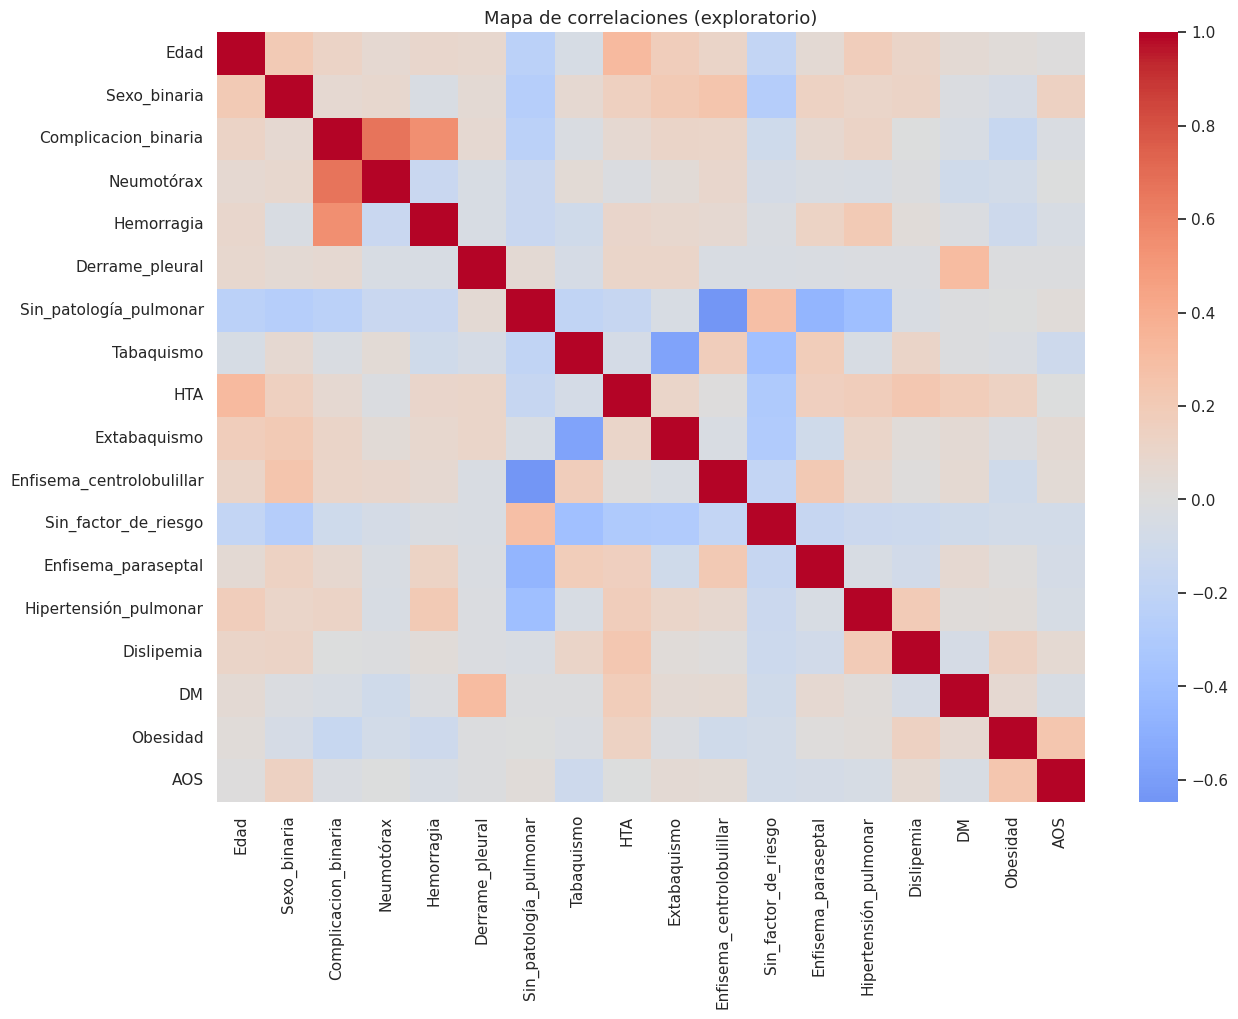
\includegraphics[width=1\textwidth]{imagenes/eda/mapa_correlaciones.png}
    \caption{Mapa de correlaciones exploratorio entre variables clínicas, variables demográficas y etiquetas de complicación.}
    \label{fig:eda_mapa_correlaciones}
\end{figure}

En conjunto, el análisis exploratorio permitió caracterizar la cohorte desde el punto de vista demográfico y clínico, identificar las variables más prevalentes, detectar variables con baja representación y confirmar el soporte desigual de las etiquetas multietiqueta. Además, permitió obtener una visión inicial de posibles patrones asociados a la aparición de cada complicación, manteniendo una interpretación descriptiva debido al tamaño limitado de la cohorte y al carácter no excluyente de las etiquetas.



\section{Preprocesamiento de los datos}
Tras el análisis de los datos, se procedió al preprocesamiento en Python de ambos tipos de datos para prepararlos para su uso en modelos. Con ello se estandarizó el formato de entrada y se redujo la variabilidad.


\subsection{Preprocesamiento de datos de volúmenes DICOM}

El preprocesamiento comprendió la implementación del \textit{pipeline} mediante MONAI, la homogeneización espacial de los volúmenes, el aumento de datos, la aplicación de ventanas de Hounsfield y la incorporación de segmentaciones anatómicas a las representaciones de entrada.

\subsubsection{Uso de MONAI en el procesamiento de imágenes médicas}

El preprocesamiento de los volúmenes DICOM se desarrolló principalmente mediante MONAI, una biblioteca basada en PyTorch y orientada al análisis y modelado de imágenes médicas \cite{cardoso2022monai}. Esta herramienta permite construir flujos de transformación de forma modular, lo que facilita definir \textit{pipelines} específicos para las fases de entrenamiento y validación. Además de las transformaciones incluidas en MONAI, se incorporaron operaciones personalizadas para adaptar el procesamiento a las características concretas de los estudios de tomografía computarizada utilizados en este trabajo.

\subsubsection{Homogeneización del tamaño de los volúmenes}

Uno de los principales retos asociados a los datos DICOM fue la variabilidad en las dimensiones de los volúmenes. Los estudios presentaban diferencias tanto en el número de cortes axiales como en la resolución espacial de cada corte, con tamaños como $512 \times 512$ o $768 \times 768$. Dado que las redes convolucionales tridimensionales requieren entradas de tamaño fijo, fue necesario redimensionar todos los volúmenes a una forma común.

Para ello, se utilizó interpolación trilineal, una técnica adecuada para datos volumétricos al tener en cuenta la continuidad espacial entre cortes y entre píxeles vecinos. Esta transformación permitió obtener entradas homogéneas sin romper la estructura tridimensional de la imagen.

Durante la fase experimental se probaron diferentes tamaños objetivo. Inicialmente, se trabajó con resoluciones elevadas, como $(256,512,512)$ o $(128,256,256)$, con el fin de conservar la mayor cantidad de información anatómica posible. No obstante, estas configuraciones implicaban un mayor coste computacional y tiempos de entrenamiento más largos. Por ello, también se evaluaron tamaños más reducidos, como $(128,128,128)$, $(64,64,64)$ e incluso $(28,28,28)$, con el objetivo de acelerar el entrenamiento y reducir el consumo de memoria. Las resoluciones más compactas permitían trabajar de forma más eficiente y facilitar la comparación entre experimentos.


\subsubsection{\textit{Data augmentation}}

Con el objetivo de mejorar la capacidad de generalización de los modelos, se incorporaron transformaciones de aumento de datos durante el entrenamiento. El aumento de datos se ha aplicado durante el entrenamiento, mientras que los volúmenes de validación se han conservado sin estas transformaciones.

Entre las transformaciones utilizadas se incluyó \texttt{RandAffine}, que permite aplicar de forma aleatoria pequeñas rotaciones, traslaciones y cambios de escala. Estas variaciones simulan diferencias razonables en el posicionamiento del paciente y en la adquisición de las imágenes. Las transformaciones se configuraron con intensidades moderadas para no alterar de forma artificial la anatomía ni introducir deformaciones no realistas, manteniendo así la coherencia clínica de los volúmenes.


\subsubsection{Aplicación de ventanas de Hounsfield}

Como se explicó en la Sección~\ref{sec:fundamentos_TC}, las intensidades de las imágenes de TC se expresan en unidades HU, lo que permite relacionar los valores de cada vóxel con la densidad radiológica del tejido. No obstante, el rango completo de HU es muy amplio, por lo que no todos los tejidos pueden visualizarse o analizarse con el mismo nivel de contraste. Por este motivo, se aplicaron ventanas de Hounsfield dentro del \textit{pipeline} de preprocesamiento, con el objetivo de resaltar rangos de intensidad clínicamente relevantes.

En el contexto de este trabajo, las ventanas se utilizaron para centrar la información de entrada en estructuras de interés para el análisis pulmonar. En particular, se emplearon configuraciones orientadas a resaltar el parénquima pulmonar y otros tejidos relevantes, recortando los valores de intensidad al rango definido por cada ventana y normalizando posteriormente el resultado al intervalo $[0,1]$. Esta normalización permite obtener una representación más homogénea entre estudios y facilita el entrenamiento de los modelos.

Se implementaron dos estrategias principales dentro del \textit{pipeline}:

\begin{itemize}
    \item \textbf{\texttt{Windowingd}}: aplica una única ventana de intensidad, como la ventana pulmonar, generando un canal de entrada centrado en un rango HU concreto.

    \item \textbf{\texttt{MultiWindowingd}}: aplica varias ventanas clínicas, como pulmón, mediastino o consolidación, y concatena los resultados como canales independientes. Esta estrategia permite proporcionar al modelo información complementaria de distintos rangos de tejido.
\end{itemize}

En la Figura~\ref{fig:hu-ejemplo} se muestra un ejemplo de la misma imagen axial de TC con distintas configuraciones de ventana. Se observa cómo el ajuste de los valores de WL y WW modifica el contraste de las estructuras pulmonares y permite destacar información anatómica diferente.

\begin{figure}[!htbp]
    \centering
    \includegraphics[width=\textwidth]{imagenes/eda/hu_ejemplos.png}
    \caption{Comparación de la misma imagen axial de TC preprocesada con diferentes configuraciones de ventana HU: sin ventana, con ventana centrada en -600 HU y ancho 1500, y con ventana centrada en -300 HU y ancho 1400. Se observa cómo el ajuste de ventana modifica el contraste de las estructuras pulmonares. Elaboración propia.}
    \label{fig:hu-ejemplo}
\end{figure}

De este modo, la aplicación de ventanas HU permite trasladar al preprocesamiento computacional una práctica habitual en radiología, donde se ajustan los rangos de visualización para destacar estructuras concretas. Además, contribuye a reducir la variabilidad de intensidades y a proporcionar al modelo una entrada más estable y orientada a la información anatómica de interés.


% \subsubsection{Segmentación anatómica}

% Con el objetivo de guiar al modelo hacia regiones anatómicas de interés, se incorporó una etapa de segmentación automática sobre los volúmenes de TC. Esta fase permitió generar máscaras específicas de distintas estructuras relevantes para el análisis pulmonar, reduciendo la influencia de regiones no relacionadas con la tarea de predicción y proporcionando al modelo información más localizada desde el punto de vista clínico.

% La segmentación se realizó mediante \texttt{TotalSegmentator} \cite{wasserthal2023totalsegmentator}, una herramienta basada en modelos de deep learning preentrenados para la segmentación automática de estructuras anatómicas en imágenes médicas. Para su aplicación, los estudios DICOM se convirtieron previamente al formato NIfTI (\texttt{.nii} o \texttt{.nii.gz}), y las máscaras resultantes se almacenaron siguiendo una nomenclatura uniforme para cada paciente.

% En concreto, se generaron diferentes tipos de segmentación, centrados en estructuras de interés para el estudio:

% \begin{itemize}
%     \item \textbf{\texttt{lung}}: segmentación del parénquima pulmonar, utilizada para delimitar la región principal de análisis.

%     \item \textbf{\texttt{nodule}}: segmentación de los nódulos pulmonares, con el objetivo de localizar las lesiones tumorales presentes en el volumen.

%     \item \textbf{\texttt{vessels}}: segmentación de los vasos pulmonares, que permite incorporar información sobre estructuras vasculares cercanas a la zona de biopsia.

%     \item \textbf{\texttt{bronquia}}: segmentación de las estructuras bronquiales, relevantes para caracterizar la anatomía pulmonar y su relación con posibles complicaciones.
% \end{itemize}

% Estas segmentaciones se ejecutaron sobre todos los volúmenes disponibles en formato NIfTI y se guardaron en directorios independientes según el tipo de estructura segmentada.

% Una vez obtenidas las máscaras anatómicas, estas se incorporaron a los experimentos de deep learning como parte de la representación de entrada de los modelos 3D. En lugar de utilizar únicamente el volumen de TC, se evaluaron distintas combinaciones de imagen y segmentaciones con el objetivo de analizar si la información anatómica explícita podía ayudar al modelo a focalizar el aprendizaje en regiones clínicamente relevantes.

% En concreto, se consideraron dos formas principales de uso de las máscaras. Por un lado, algunas configuraciones utilizaron volúmenes de TC enmascarados, en los que la imagen se restringe a una región anatómica concreta, como el pulmón o el nódulo. Este planteamiento dio lugar a entradas como \texttt{lung\_only\_masked\_ct} y \texttt{nodule\_only\_masked\_ct}, orientadas respectivamente a conservar la información contenida dentro de la máscara pulmonar o dentro de la máscara del nódulo. Por otro lado, se evaluaron representaciones multicanal en las que la imagen de TC se combinó con una o varias máscaras binarias como canales adicionales. En este grupo se incluyeron configuraciones como \texttt{ct\_lung\_nodule}, \texttt{nodule\_vessels} y \texttt{ct\_lung\_nodule\_vessels}, que incorporan de forma explícita la localización del pulmón, el nódulo y las estructuras vasculares.

% Esta estrategia permitió comparar si el rendimiento predictivo dependía únicamente de la intensidad de la imagen o si mejoraba al proporcionar al modelo información estructural derivada de las segmentaciones. De este modo, las máscaras no se utilizaron como variables de salida, sino como una forma de guiar la representación de entrada hacia estructuras relacionadas con el procedimiento de biopsia y con el riesgo potencial de complicaciones.

\subsubsection{Segmentación anatómica}

La generación de las máscaras anatómicas descritas en el Capítulo~\ref{chap:planteamiento_problema} requirió convertir previamente los estudios DICOM al formato NIfTI. Para las segmentaciones automáticas se utilizó \texttt{TotalSegmentator} \cite{wasserthal2023totalsegmentator}, una herramienta basada en modelos de \textit{deep learning} preentrenados para la delimitación de estructuras anatómicas en imágenes médicas.

Las máscaras resultantes se almacenaron en directorios diferenciados según la estructura representada y siguiendo una nomenclatura uniforme para cada paciente. Durante su preparación se mantuvo la correspondencia espacial entre cada máscara y su volumen de TC, necesaria para aplicar el enmascaramiento de las imágenes, extraer características radiómicas y construir entradas multicanal. Las formas concretas de incorporación de estas máscaras a los modelos se describen en los capítulos experimentales correspondientes.

\subsection{Preprocesamiento de los datos tabulares}

El preprocesamiento de los datos clínicos tabulares ha tenido como objetivo adaptar la información disponible a un formato adecuado para la tarea de clasificación. Para ello, se han empleado las bibliotecas \textit{pandas} y \textit{scikit-learn} de Python para manipular los datos y aplicar las transformaciones necesarias.

En primer lugar, se han eliminado las columnas que no se iban a utilizar en los modelos, entre ellas \textit{Tipo de cáncer}, ya que el estudio se ha centrado en predecir y caracterizar las complicaciones clínicas registradas. Posteriormente, se han transformado las variables con formato multietiqueta: \textit{Tipo de complicación}, \textit{Factor de riesgo} y \textit{Patología pulmonar}. Dado que estas variables podían contener varias categorías para un mismo paciente, se han codificado mediante una representación binaria multietiqueta utilizando \texttt{MultiLabelBinarizer} de \textit{scikit-learn}. En la variable \textit{Tipo de complicación}, los valores ausentes o marcados con \textit{X} se han interpretado como ausencia simultánea de hemorragia y neumotórax, representada mediante el conjunto vacío de etiquetas y no como una etiqueta independiente. En las variables descriptivas, la ausencia de antecedentes se ha representado mediante categorías explícitas, como \textit{Sin\_factor\_de\_riesgo} y \textit{Sin\_patología\_pulmonar}.

También se ha normalizado la variable \textit{Edad} en el rango $[0,1]$ utilizando \texttt{MinMaxScaler}, con el fin de evitar diferencias de escala respecto al resto de las variables numéricas. Por último, se han codificado las variables categóricas necesarias para el entrenamiento, incluida la transformación de \textit{Sexo} en una variable binaria. La variable \textit{Tipo de complicación} se ha transformado en las etiquetas de hemorragia y neumotórax. Los pacientes sin ninguna de estas complicaciones han quedado representados mediante la ausencia de ambas etiquetas, mientras que el indicador global de complicación se ha conservado únicamente como referencia descriptiva. Como resultado, se ha obtenido un conjunto de datos clínicos limpio, compuesto por variables numéricas y binarias, preparado para su análisis posterior y su incorporación a los modelos predictivos.

\subsection{Resumen de las cohortes experimentales}
\label{subsec:resumen_cohortes}

La disponibilidad de las distintas fuentes de información no ha sido uniforme para todos los pacientes. Por este motivo, cada bloque experimental se ha realizado sobre la intersección de casos que disponía de las entradas necesarias para el análisis correspondiente. La Tabla~\ref{tab:resumen_cohortes} resume las principales cohortes utilizadas. Los conjuntos no deben interpretarse únicamente como reducciones sucesivas de una misma muestra, ya que algunos se han definido mediante criterios de disponibilidad específicos de cada representación.

\begin{table}[!htbp]
\centering
\small
\renewcommand{\arraystretch}{1.15}
\caption{Resumen de las principales cohortes y subconjuntos empleados en el estudio. \(N\) indica el número de pacientes.}
\label{tab:resumen_cohortes}
\begin{tabularx}{\textwidth}{p{4.0cm}cX}
\toprule
\textbf{Cohorte o bloque} & \(\boldsymbol{N}\) & \textbf{Criterio de disponibilidad o finalidad} \\
\midrule

Cohorte clínica inicial
& 210
& Pacientes con información clínica anonimizada, utilizados para la caracterización descriptiva inicial y como base del análisis clínico de descubrimiento de subgrupos. \\

Cohorte con TC principal
& 209
& Pacientes con un estudio DICOM principal válido y correctamente relacionado con la información clínica. \\

Cohorte multietiqueta elegible
& 209
& Pacientes considerados para la formulación basada en hemorragia y neumotórax tras excluir del modelado el caso que presentaba únicamente derrame pleural. \\

% Radiómica
% & 206
% & Pacientes con información clínica y representaciones de imagen y segmentación utilizables para la extracción y el análisis de características radiómicas. \\
Radiómica disponible
& 206
& Pacientes con una extracción radiómica utilizable \\

Clasificación radiómica
& 205
& Pacientes con características radiómicas y etiquetas completas de hemorragia y neumotórax \\

Aprendizaje profundo y PU tridimensional
& 204
& Pacientes con etiquetas, volúmenes preprocesados y máscaras requeridas por las entradas tridimensionales. Esta cohorte también se ha utilizado en los experimentos multimodales y de transferencia de aprendizaje. \\

PU learning tabular
& 205
& Intersección empleada para comparar las representaciones clínicas y geométricas, radiómicas y combinadas dentro del análisis tabular de PU learning. \\

Descubrimiento de subgrupos con geometría
& 201
& Pacientes con medidas geométricas completas del tamaño nodular y de la profundidad respecto a la pleura, utilizados en las representaciones emparejadas. \\

% Análisis SHAP de R07
% & 195
% & Pacientes incluidos en las predicciones OOF de la configuración R07 y explicados mediante el modelo correspondiente a su \textit{fold} externo. \\
Análisis SHAP de R07
& 205
& Pacientes incluidos en las predicciones OOF de la configuración R07 y explicados mediante el modelo correspondiente a su \textit{fold} externo. \\

\bottomrule
\end{tabularx}
\end{table}

Cuando se ha comparado directamente el efecto de distintas representaciones dentro de un mismo experimento, todas las alternativas han utilizado los mismos pacientes y la misma asignación a los conjuntos de entrenamiento y prueba. De este modo, las diferencias observadas no se deben a cambios en la composición de la cohorte o de las particiones. 
